\documentclass[a4paper,12pt,titlepage]{article}
\usepackage[T1]{fontenc}
\usepackage[utf8]{inputenc}
\usepackage[italian]{babel}
\usepackage[]{frontespizio}

\usepackage[hidelinks]{hyperref}

\usepackage{geometry}
\usepackage{graphicx}
\usepackage{float}

\graphicspath{ {./images/} }


\begin{document}
\begin{frontespizio}
	\Universita{Verona}
	\Facolta{Scienze ed Ingegneria}
	\Corso[laurea triennale]{Informatica}
	\Annoaccademico{2018-2019}
	\Titolo{Relazione ingegneria del software}
	\Logo[4cm]{logo.png}
	\Candidato[VR421663]{Marchiotto Nicola}
	\Candidato[VR422112]{Gugole Nicola}
\end{frontespizio}


\clearpage
\null
\thispagestyle{empty}
\clearpage

%Indice
\tableofcontents
\thispagestyle{empty}

\clearpage
\null
\thispagestyle{empty}
\clearpage

\setcounter{page}{1}

\section{Requisiti}\label{sec:requisiti}
Si vuole progettare un sistema informatico per gestire gli acquisti on-line di una libreria.
Per ogni libro si memorizza il titolo, l’autore o gli autori, la casa editrice, l’anno di pubblicazione, il
codice ISBN (identificativo), il genere, il prezzo ed una breve descrizione. Gli utenti possono
visualizzare le classifiche di vendita che sono organizzate per genere (novità, narrativa, ragazzi, …)
e vengono aggiornate ogni settimana. Per ogni posizione della classifica si indica da quante
settimana il libro è in quella posizione.\\
Il sistema memorizza gli ordini degli utenti. Gli utenti possono essere registrati o meno. Per gli
utenti si memorizzano nome, cognome, indirizzo, CAP, città, numero di telefono ed email. Ogni
utente registrato accede con email e password ed ha associata una LibroCard per la raccolta punti.
Ogni LibroCard ha un numero identificativo, una data di emissione e il totale dei punti raccolti. Gli
utenti registrati possono specificare uno o più indirizzi di spedizione diversi da quello di residenza.
Ogni libro ha associato il numero di punti che vengono caricati sulle LibroCard in caso di acquisto
da parte di utenti registrati.\\
Per ogni ordine si memorizzano il codice (univoco), la data, i libri che lo compongono, l’utente che
lo ha effettuato, il costo totale, il tipo di pagamento (carta di credito, paypal o contrassegno) e il
saldo punti se l’utente è registrato.\\
Il sistema deve permettere agli utenti registrati di accedere al loro profilo, modificare i dati
anagrafici, verificare il saldo punti e lo stato dei loro ordini. Ogni utente registrato può vedere tutti
gli ordini che ha effettuato nel tempo con il totale dei punti accumulati per ogni ordine.
Gli utenti non registrati possono accedere agli ordini cha hanno effettuato tramite il codice
dell’ordine.\\\
I responsabili della libreria devono poter verificare lo stato degli ordini, e il saldo punti delle
LibroCard degli utenti registrati.\\
Inoltre, i responsabili della libreria sono responsabili dell’inserimento dei dati relativi ai libri che si
possono ordinare e dell’aggiornamento delle classifiche.\\
Tutti gli utenti sono opportunamente autenticati dal sistema per poter accedere alle funzionalità
di loro competenza.

\cleardoublepage

\section{Ingegneria e sviluppo}\label{sec:ingegneria e sviluppo}
Di seguito riportiamo le decisioni concernenti la realizzazione dell’interfaccia grafica, il salvataggio
delle informazioni sui libri e sugli utenti della libreria, e dei pattern architetturali, comportamentali
e creazionali.

\subsection{Organizzazione iniziale}
Al fine di ottimizzare il lavoro di squadra, ogni membro si è specialiazzato in un aspetto specifico del progetto. Marchiotto N. si è occupato della creazione dell'interfaccia grafica considerando gli aspetti e/o modi con cui gli utenti si
aspettano di interagire con il sistema e quindi di sviluppare accordatamente una GUI generale. Data la forte connessione tra la parte di interfaccia e i relativi controllori, Marchiotto N. si è occupato anche dello sviluppo dei controllori e dei modelli dei componenti, i quali si identificano in parte preponderante il pattern MVC.
Gugole N. si è invece occupato della progettazione e sviluppo della parte back-end, gestendo il database nonchè lo sviluppo della comunicazione con il sistema e l'implementazione dei metodi necessari a ricevere i dati il più comodamente possibile in Java.


\subsection{Software e strumenti utilizzati}

\textbf{Interfaccia grafica: }La nostra scelta di linguaggio di programmazione e ricaduta su \textit{Java} e conseguentemente su \textit{JavaFX}, non abbiamo utilizzato le componenti \textit{Swing} in quanto poco utilizzate nel mondo odierno temendo una futura possibile poca portabilità del codice su altre piattaforme.
Inoltre un altro aspetto interessante di JavaFX è la facilità con cui viene implementato il pattern architetturale MVC
da noi appunto adottato. Infine ci siamo avvalsi dell’ausilio del tool Scene Builder che permette di costruire visualmente ed
in modo molto semplice un’interfaccia grafica tramite la generazione automatica dei file FXML, i quali separano la progettazione grafica di una “scena” dalla logica funzionale ad essa legata.\\

\textbf{Dababase: }Dopo una ricerca effettuata in comune (vista la nostra ignoranza in materia di DataBase, ancora per qualche mese), la scelta è ricaduta sull'uso del linguaggio \textit{SQLite}, linguaggio più semplice e con meno opzioni del suo compagno \textit{MySQL}, ma con tutto ciò che serve al fine di questo progetto. Per avere una miglior interpretazione di cosa effettivamente accada all'interno del nostro DataBase ci siamo affidati ad un software grafico ed opensource per la visualizzazione e la possibile modifica dello stesso: \textit{DB Browser}.\\

\textbf{Gestione codice: }Data la natura di sviluppo adotta nel nostro progetto, ovvero incrementale basata su un approccio agile, è sorta subito la necessità di scambio di codice tra i due componenti in modo intuitivo e veloce. Tale necessità è stata risolta tramite la piattaforma \textit{GitHub}, data la sua ubiquità e portabilità, installato localmente sulle macchine dei membri del team e riferente una repository remota privata localizzata su Github.\\

\subsection{Pattern}\label{sec:pattern}
Dopo aver letto attentamente la specifica e aver redatto lo schema dei casi d’uso provvisorio, si sono discussi diversi possibili approcci e in particolare si è cercato di determinare se e quali design patterns fossero più adatti da usare al fine di costruire il
sistema generale.\\ Per il nostro sistema abbiamo fatto uso prevalentemente del design pattern \textit{Model View Controller (MVC)}, il quale specifica che un'applicazione sia composta da un \textit{Model}, il quale contiene solo dati puri senza nessuna conosceza su come rappresentare tali dati all'utente, da una \textit{View}, la quale rappresenta il sistema all'utente ma che non sa come manipolare i dati e gli input forniti da quest'ultimo, e da una parte \textit{Controller}, quest'ultima esiste tra la \textit{View} e il \textit{Model}, cattura gli eventi generati dalla \textit{View} e reagisce in modo appropriato a tali eventi. In molti casi la reazione consiste nel richiamare un metodo sul \textit{Model}. Dato che la \textit{View} e il \textit{Model} sono connessi tramite un meccanismo di notifica, il risultato di queste azioni hanno un riscontro automatico sulla \textit{View}

\begin{figure}[H]
		\centering
		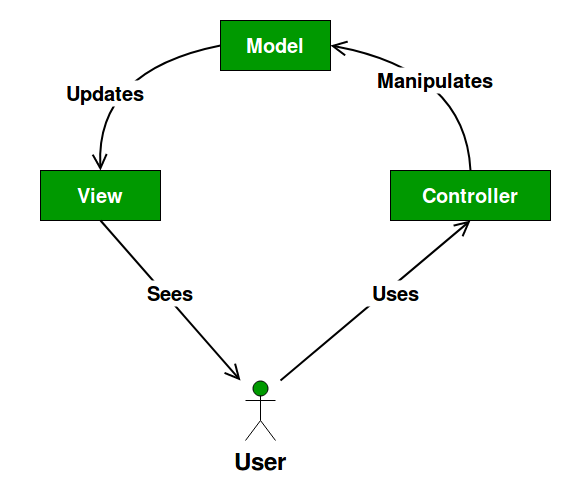
\includegraphics[scale=0.45]{MVC}
\end{figure}

Abbiamo inoltre utilizzato un pattern strutturale non trattato a lezione, ma a nostro parere particolarmente azzeccato a questa tipologia di progetto: \textit{DAO}, ovvero \textit{Data Access Object pattern.}\\
Il \textit{DAO} permette di separare completamente lo strato applicativo del programma dallo strato di acquisizione dati, non mostrando al lato di alto livello le complesse operazioni per costruire, eseguire e salvare come sono le query, etc. Tutto ciò permette ai due strati di evolvere completamente indipendentemente.\\
E' dunque una specializzazione del pattern Facade, applicata alla presenza dei DataBase.\\
\textit{DAO} è utile anche nel caso di refactoring. Il fatto di isolare completamente la gestione di tutte le interazioni con il DataBase ci permette all'occorrenza di poter cambiare ciò che serve, addirittura il linguaggio di programmazione delle query, senza che lo strato più ad alto livello si accorga di qualcosa.\\


\subsection{Scelte progettuali}\label{sec:scelte progettuali}

Di seguito riportiamo le nostre scelte progettuali in merito a passaggi di dubbia interpretazione nella consegna 
e/o limiti progettuali a cui siamo dovuti scendere.\\


\textbf{Aggiornamento classifica:}\underline{Per un'utile demo del software}, non è pensabile che l'utente debba aspettare 7 giorni per un aggiornamento settimanale, abbiamo quindi pensato di aggiornare la classifica al passaggio di X minuti rispetto ad una data di riferimento presente nel database.
Se all'avvio del programma quella data e quella di avvio del programma differiscono di più di X minuti allora avviene un aggiornamento di classifica e la data di riferimento viene aggiornata al più vicino aggiornamento teorico. Tale vincolo può essere facilmente modificato in pochi minuti, fatto in modo da non compromettere l'utilizzabilità del sistema in situazioni reali.
Il responsabile può comunque aggiornare le classifiche a suo piacimento all'interno dell'area responsabili.
L'aggiornamento responsabili è comunque leggermente differente rispetto quello settimanale,
infatti esso è fatto in modo da aggiornare le tabelle non compromettendo l'aggiornamento settimanale successivo,
non azzerando quindi i conteggi di vendita per esempio, che vanno invece azzerati ad inizio di ogni settimana.
Importante sottolineare che le classifiche nel sistema sono ordinate tramite numero di copie vendute.\\

\textbf{Stato dell'ordine:} Non potendoci basare su un sistema di consegna reale, per dare un mino di riscontro nel sistema, consideriamo un'ordine \textit{non ancora spedito} se non è passata un'ora dalla sua creazione,
dopo la prima ora l'ordine diventa \textit{spedito}, infine l'ordine è \textit{consegnato}  dalla seconda ora in poi.\\

\textbf{Accesso degli admin:} Basandoci sulle nostre poche nozioni in materia, sappiamo che i veri e 
propri admin di molti siti/sw non si possono "iscrivere", ma devono essere inseriti nel sistema. 
E così abbiamo operato anche noi: il nostro admin (credenziali admin, root) è inserito direttamente 
all'interno del DB ed il sistema lo riconosce come admin semplicemente perché è un utente esistente ma con LibroCard nulla,
eventuali altri responsabili potranno essere inseriti sempre attraverso il database alla condizione che il campo LibroCard risulti nullo.\\

\textbf{Eliminazione libri dal sistema: }Se un responsabile dovesse eliminare un libro dalla libreria, esso non sparirebbe davvero dal sistema in quanto potrebbe essere che tale libro facesse parte di un ordine di qualche utente. Tale libro viene invece marcato come non disponibile, non verrà più visualizzato nel catalogo della libreria ma sarà comunque visibile in un eventuale storico ordini dell'utente. Importante notare che il responsabile non potrà inserire nel sistema un libro con uguale titolo,autore e casa editrice a quello di un libro eliminato in quanto in realtà esso è ancora presente nel DB. Per eseguire questa operazione si dovrà intervenire direttamente nel DB e rimuovere forzatamente la entry del libro non disponibile.

\cleardoublepage

\section{Use case}\label{sec:casiduso}
Data la natura didattica del progetto non si sono seguite le classiche tecniche di ingegneria dei requisiti ma essi sono stati ricavati e studiati a partire dalla specifica di consegna, considerata, almeno in parte, come documento dei requisiti.
Nel corso dello sviluppo del progetto, a seconda delle diverse funzionalità da implementare,
sono anche stati stilati diversi casi d’uso per i vari utenti secondo un processo simile a quello
adottato dai modelli agili.\\
Di seguito parte dei casi d’uso utilizzati.
\vspace{0.3cm}
	{\renewcommand\arraystretch{1.5}{
	\renewcommand\tabcolsep{0pt}{
	\begin{table}[H]			
			
			\begin{tabular}{p{5cm} p{10cm} }
			\hline
			\textbf{Attore} & \textbf{Utente registrato} \\ \hline
			\textbf{Precondizioni} & L'utente deve essere registrato nel sistema\\ \hline
			\textbf{PostCondizioni}&  \\ \hline
			\textbf{Main path} &  - Modificare dati personali\\ 
			& - Visualizzare i propri ordini\\
			& - Aggiungere/togliere indirizzi di spedizione \\
			& - Visualizzare in dettaglio i libri\\
			& - Comprare libri\\
			& - Visualizzare le classifiche di vendita\\
			& - Eliminare il proprio account \\ \hline
			 \end{tabular}
		\end{table}
	}}
\vspace{0.3cm}
	{\renewcommand\arraystretch{1.5}{
	\renewcommand\tabcolsep{0pt}{
	\begin{table}[H]			
			\begin{tabular}{p{5cm} p{10cm} }
			\hline
			\textbf{Attore} --& \textbf{Utente non registrato} \\ \hline
			\textbf{Precondizioni} & Accedere al sistema come Guest\\ \hline
			\textbf{PostCondizioni} &  \\ \hline
			\textbf{Main path} & - Comprare libri\\
			& - Cercare e visualizzare i propri ordini tramite Id ordine\\
			& - Visualizzare in dettaglio i libri\\
			& - Visualizzare le classifiche di vendita\\ \hline
			 \end{tabular}
		\end{table}
	}}

\begin{figure}[H]
		\centering
		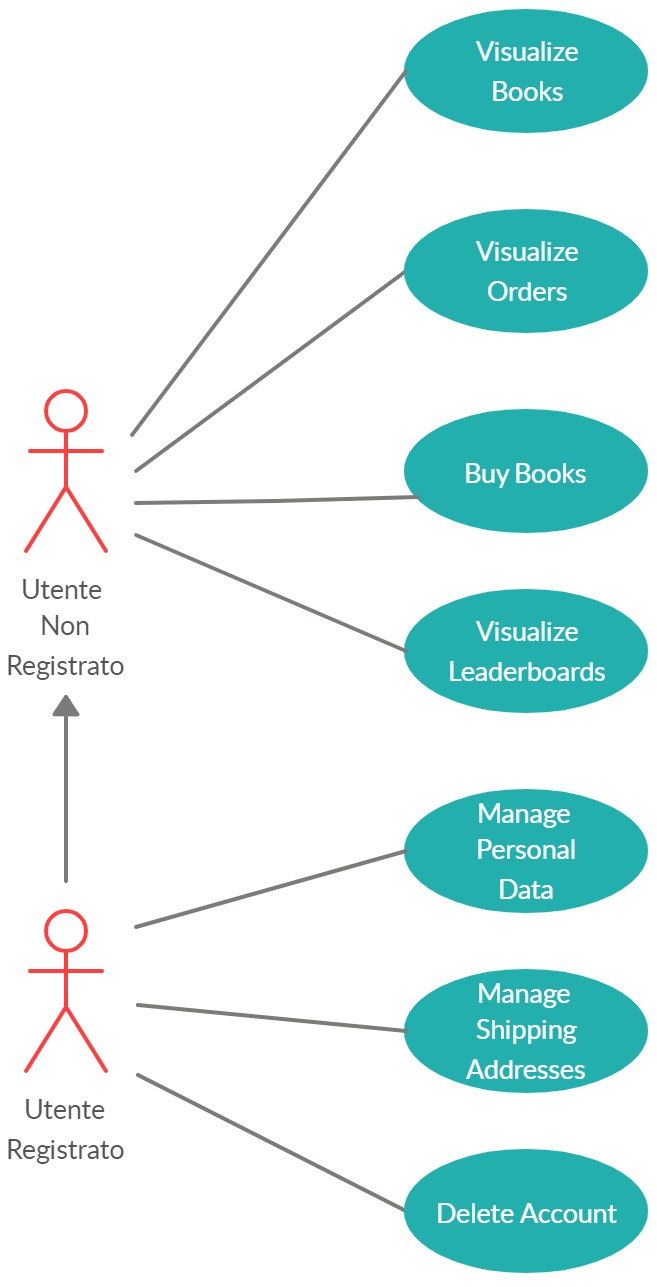
\includegraphics[scale=0.42]{useCaseUser}
		\caption{Diagramma UML dei casi d'uso dell'utente, registrato e non }
\end{figure}

\vspace{0.3cm}
	{\renewcommand\arraystretch{1.5}{
	\renewcommand\tabcolsep{0pt}{
	\begin{table}[H]			
			\begin{tabular}{p{5cm} p{10cm} }
			\hline
			\textbf{Attore} & \textbf{Responsabile} \\ \hline
			\textbf{Precondizioni} & Accedere al sistema con credenziali Responsabile\\ \hline
			\textbf{PostCondizioni} &  \\ \hline
			\textbf{Main path} & - Inserire/eliminare libri\\
			& - Visualizzare LibroCard\\
			& - Visualizzare gli ordini degli utenti\\
			& - Aggiornare le classifiche di vendita\\ \hline
			 \end{tabular}
		\end{table}
	}}
\vspace{1cm}
\begin{figure}[H]
		\centering
		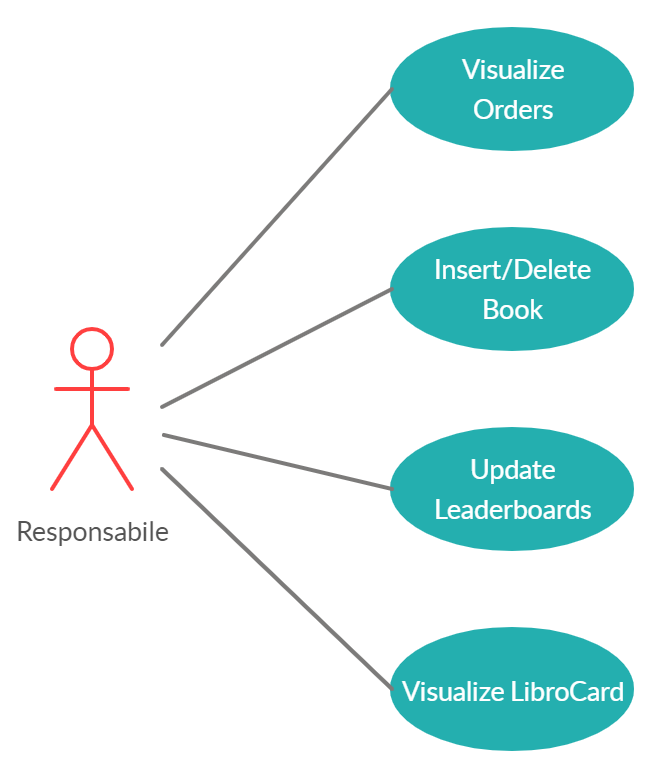
\includegraphics[scale=0.75]{useCaseResponsabile}
		\caption{Diagramma UML dei casi d'uso del responsabile }
\end{figure}


\section{Activity diagram}\label{sec:activitydiagram}
\begin{figure}[H]
		\centering
		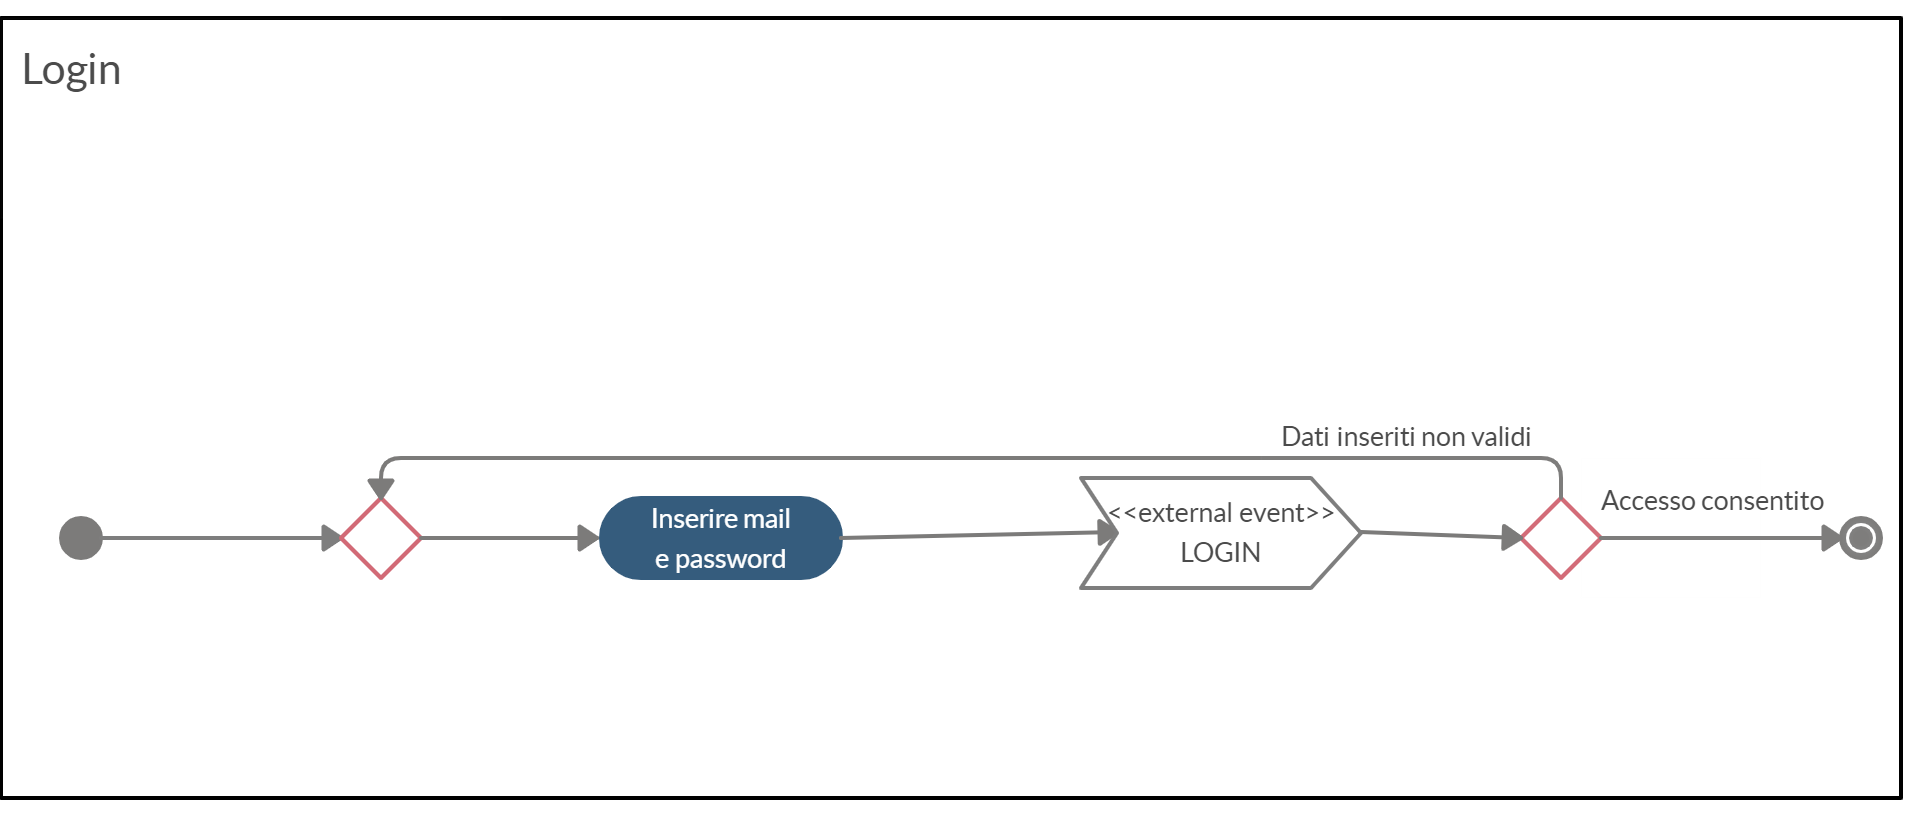
\includegraphics[scale=0.35, angle=90]{activityDiagramLogin}
		\caption{\textit{Activity diagram} dell'operazione di Login}
\end{figure}
\begin{figure}[H]
		\centering
		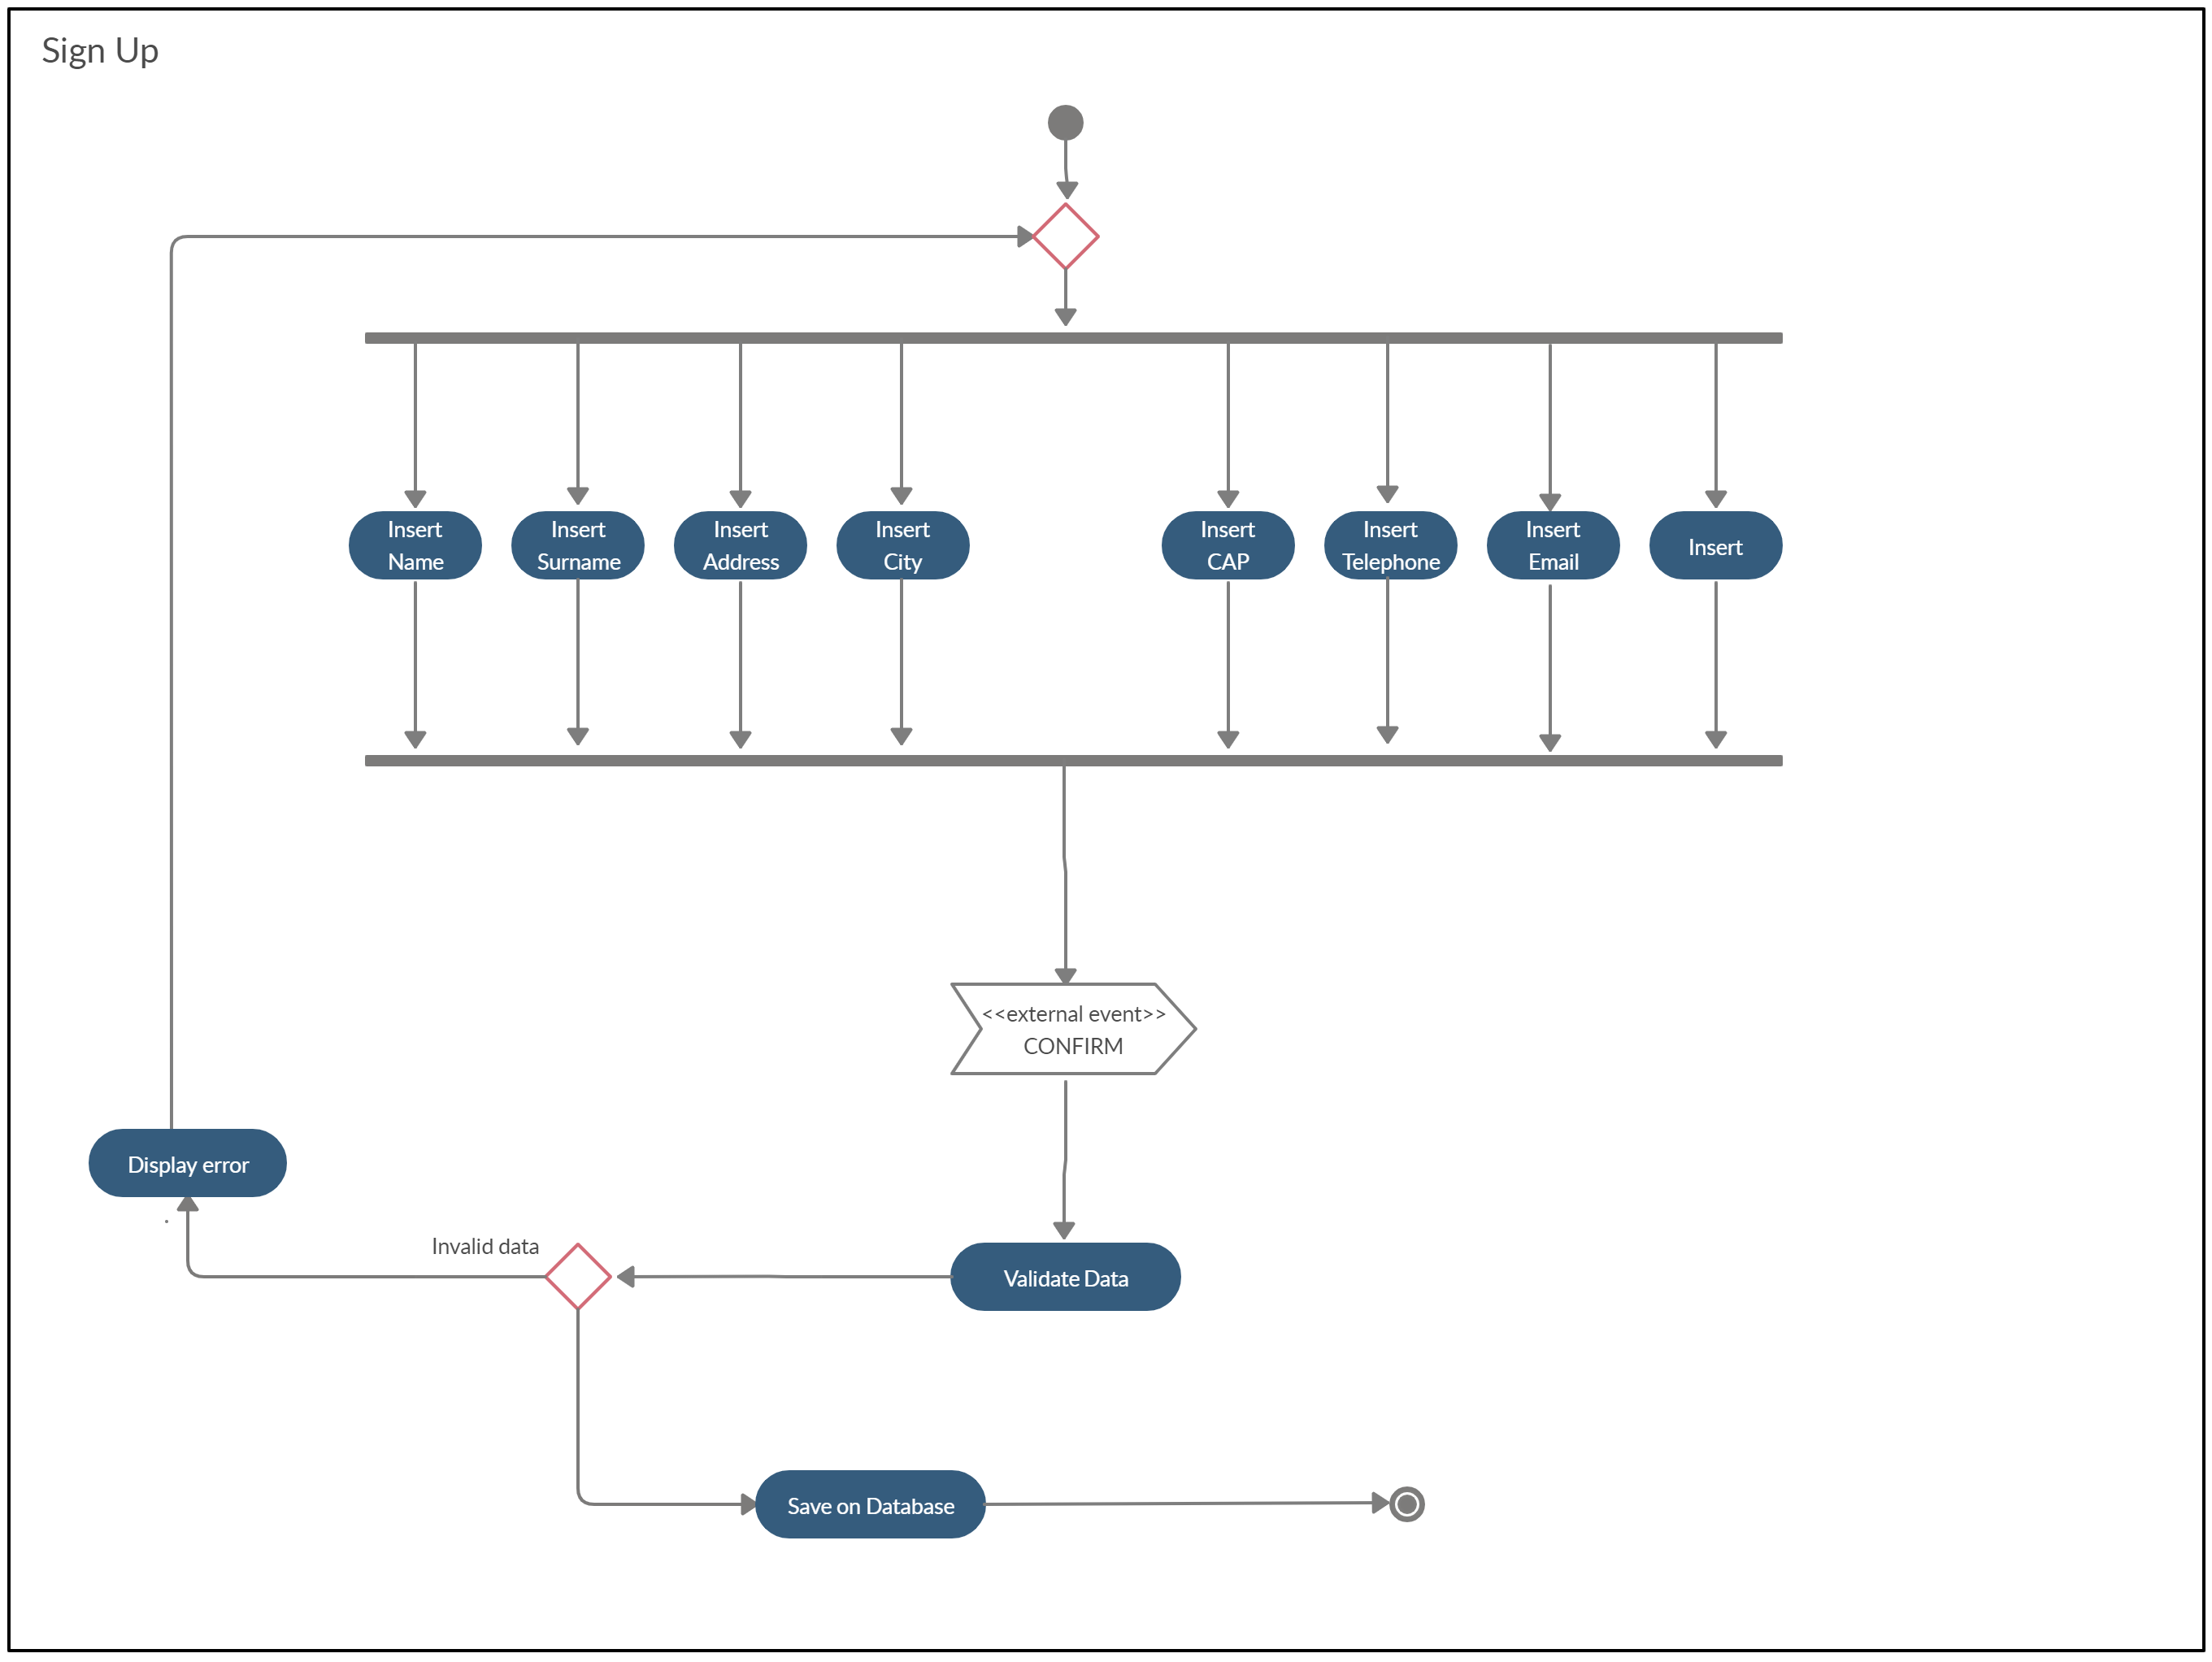
\includegraphics[scale=0.34, angle=90]{activityDiagramSignUp}
		\caption{\textit{Activity diagram} dell'operazione di SignUp}
\end{figure}
\begin{figure}[H]
		\centering
		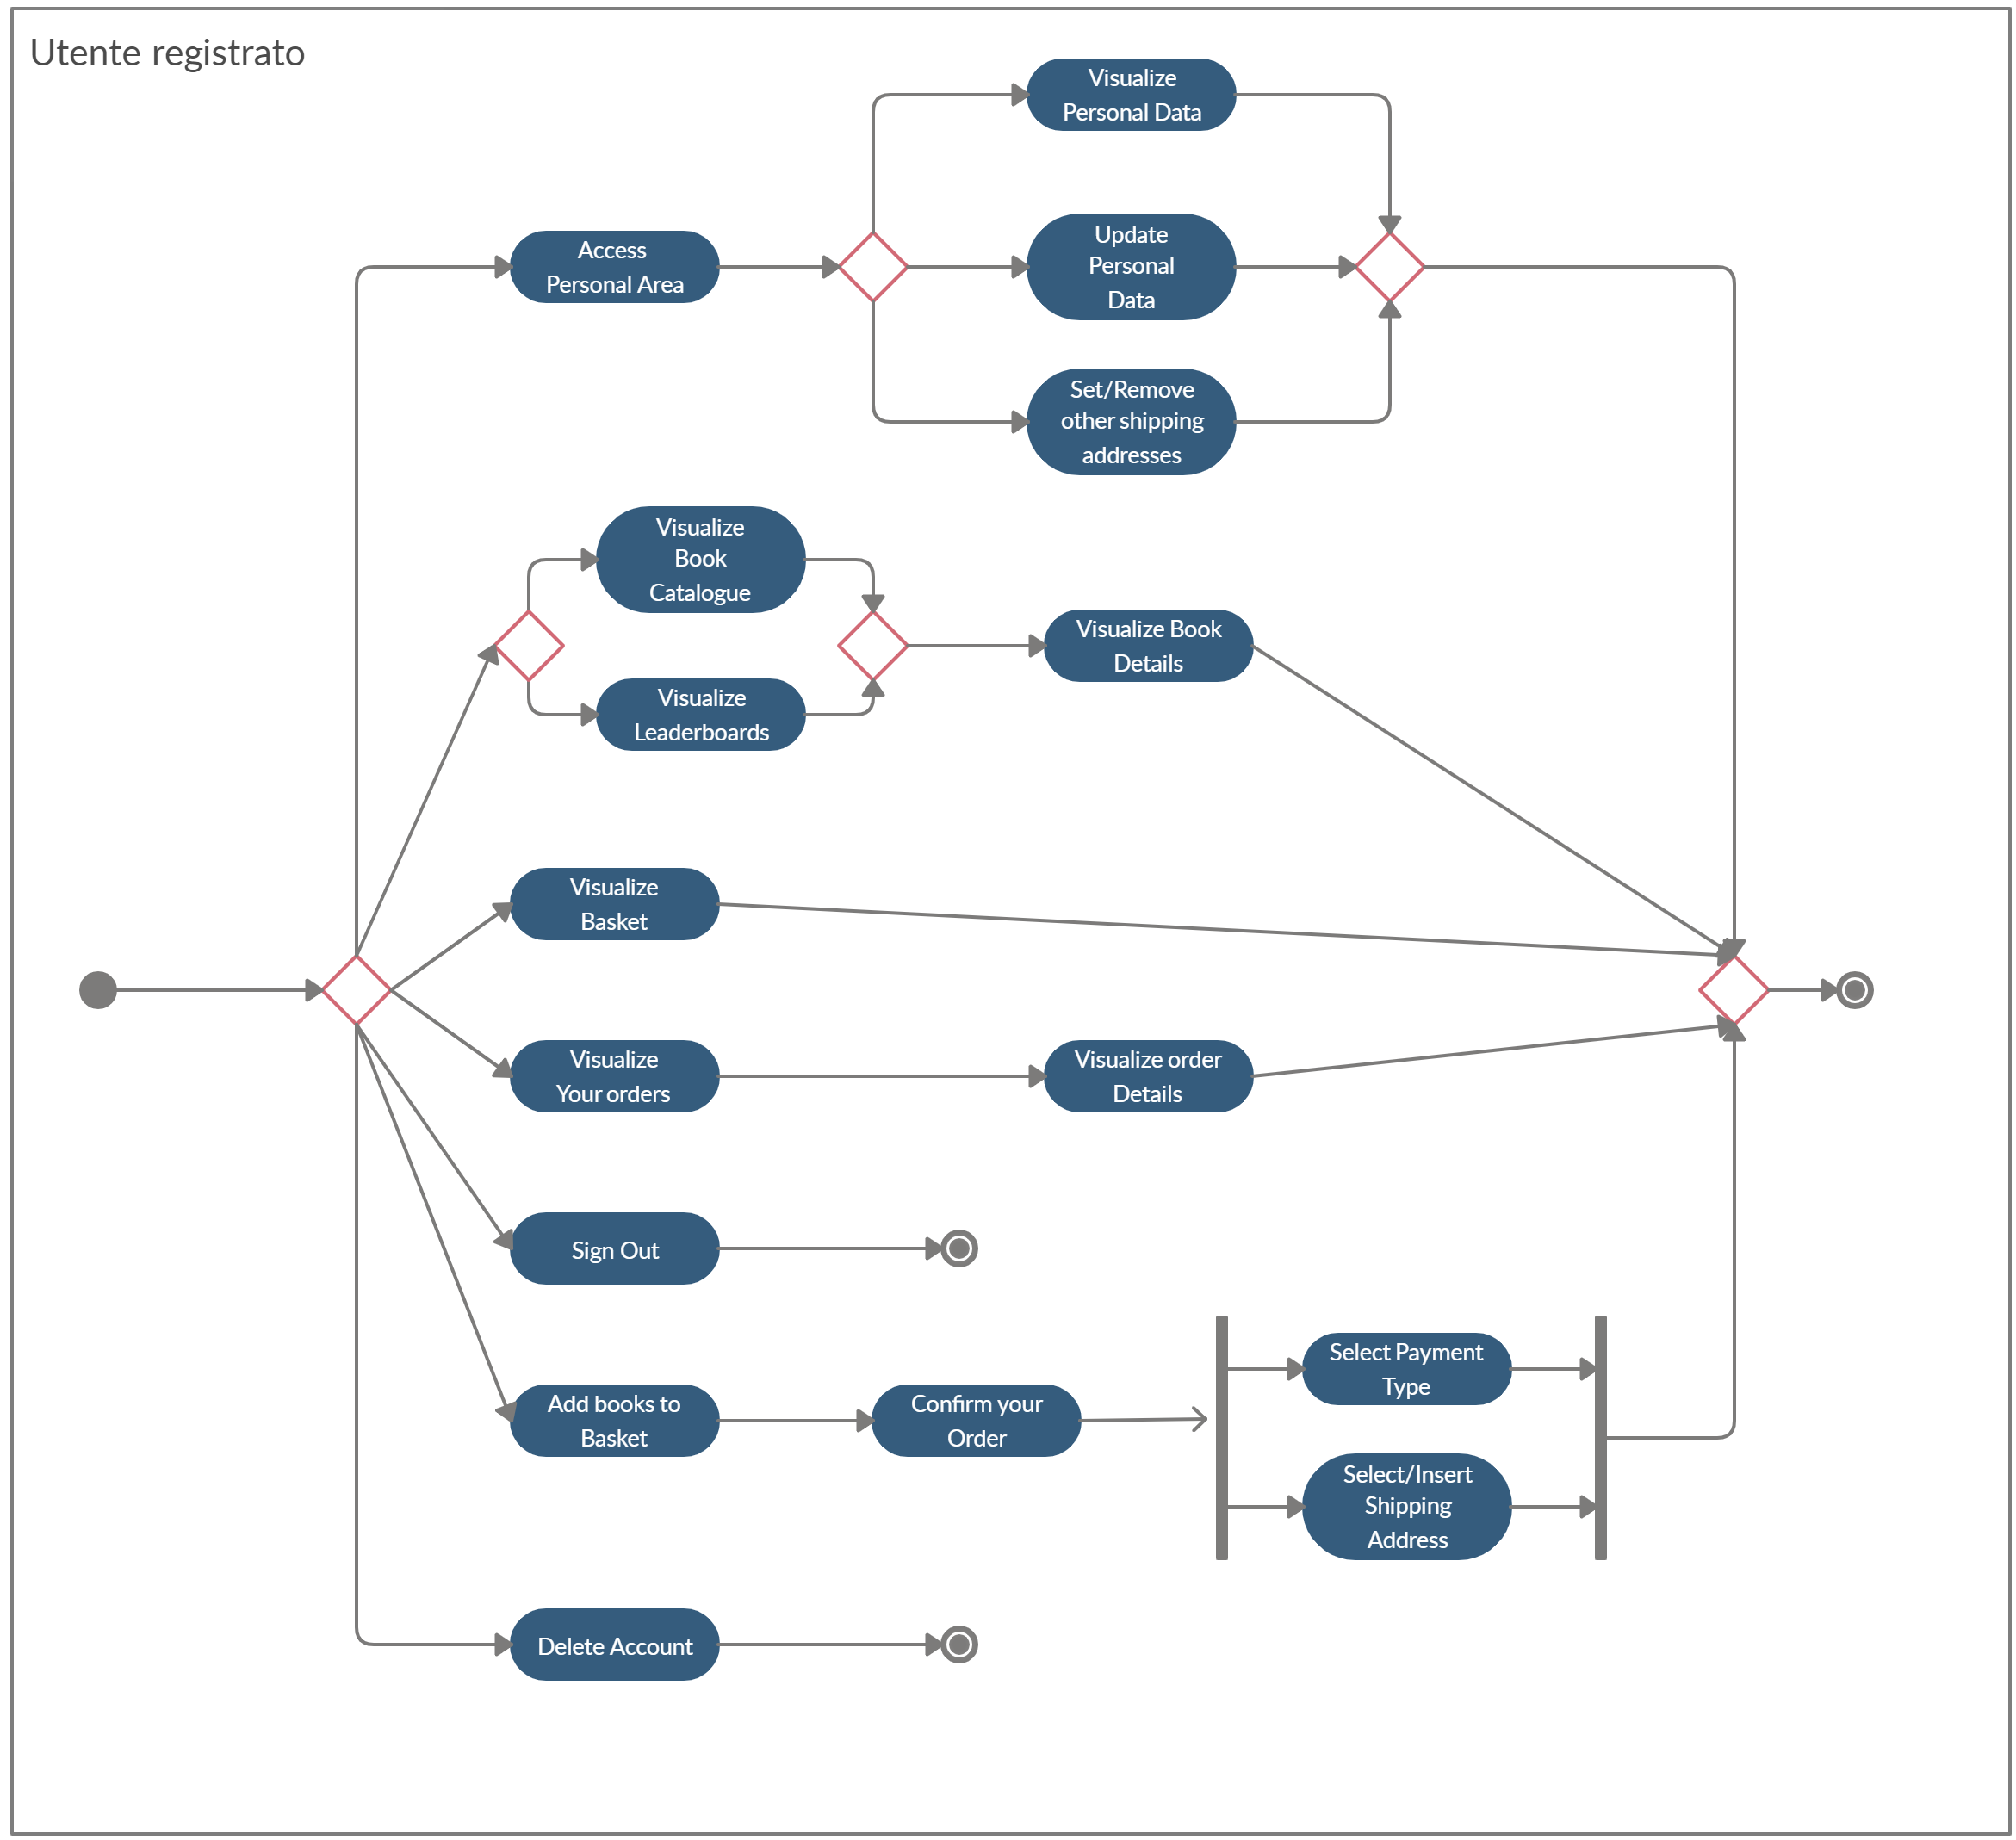
\includegraphics[scale=0.35, angle=90]{activityDiagramRegistrato}
		\caption{\textit{Activity diagram} delle diverse azioni che possono essere compiute dall'utente registrato}
\end{figure}
\begin{figure}[H]
		\centering
		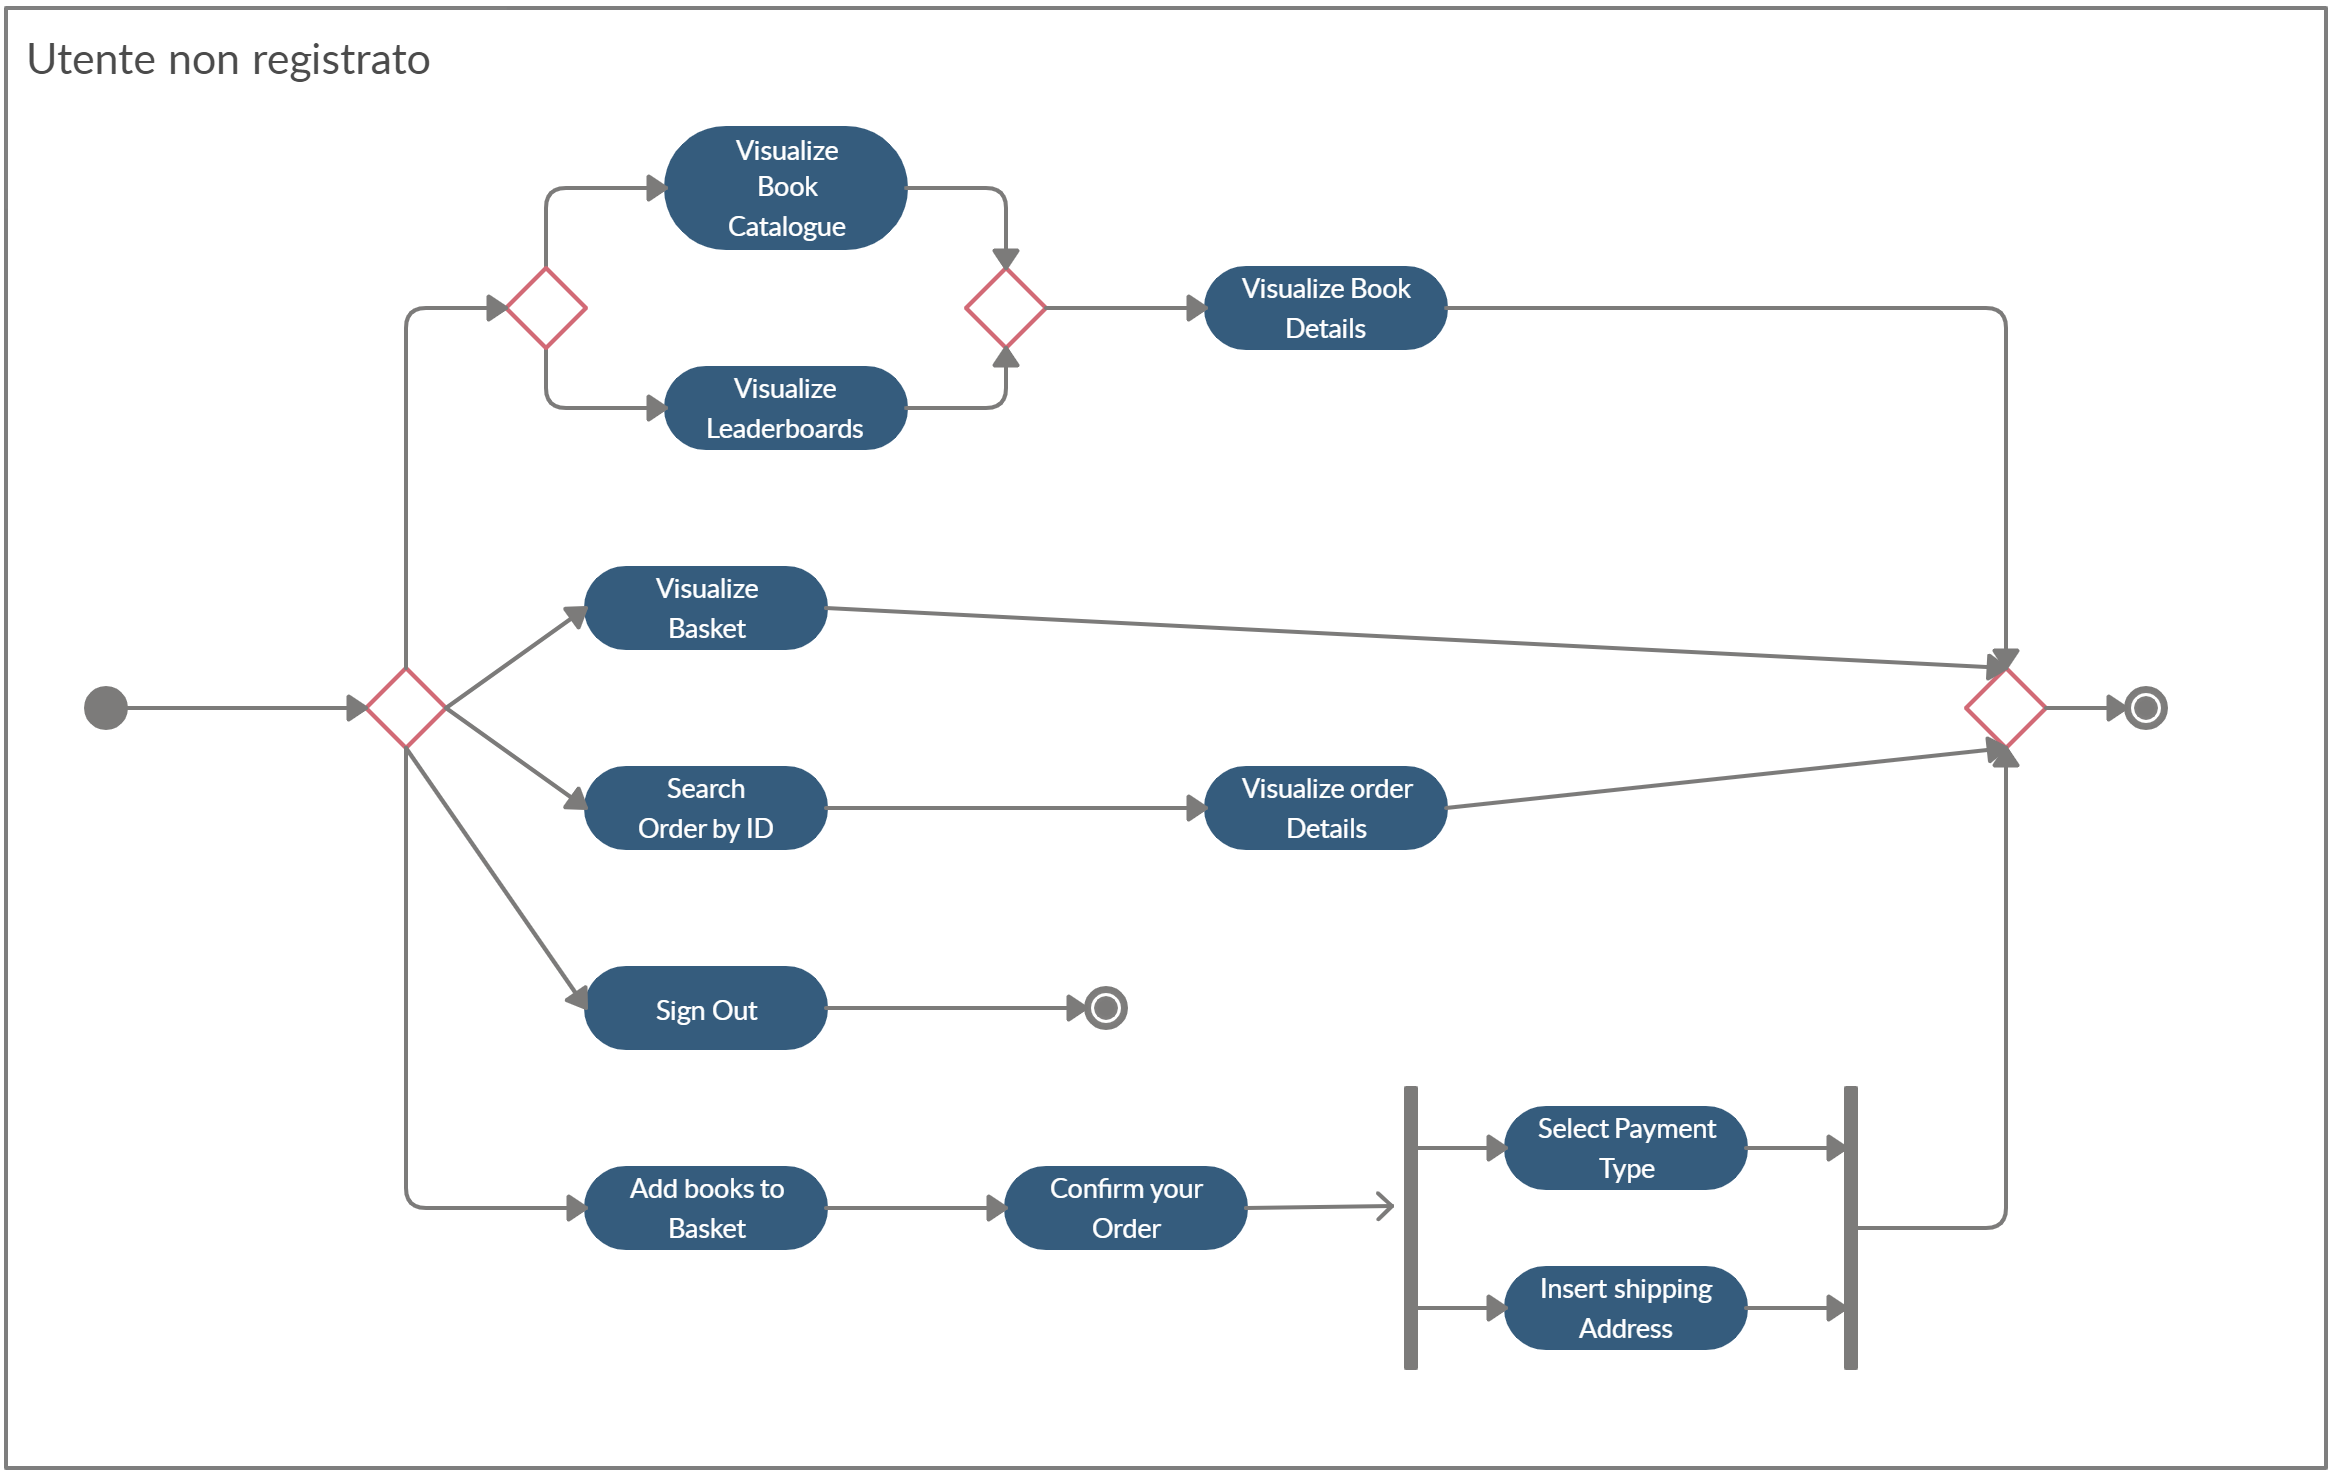
\includegraphics[scale=0.4, angle=90]{activityDiagramNonRegistrato}
		\caption{\textit{Activity diagram} delle diverse azioni che possono essere compiute dall'utente non registrato}
\end{figure}
\begin{figure}[H]
		\centering
		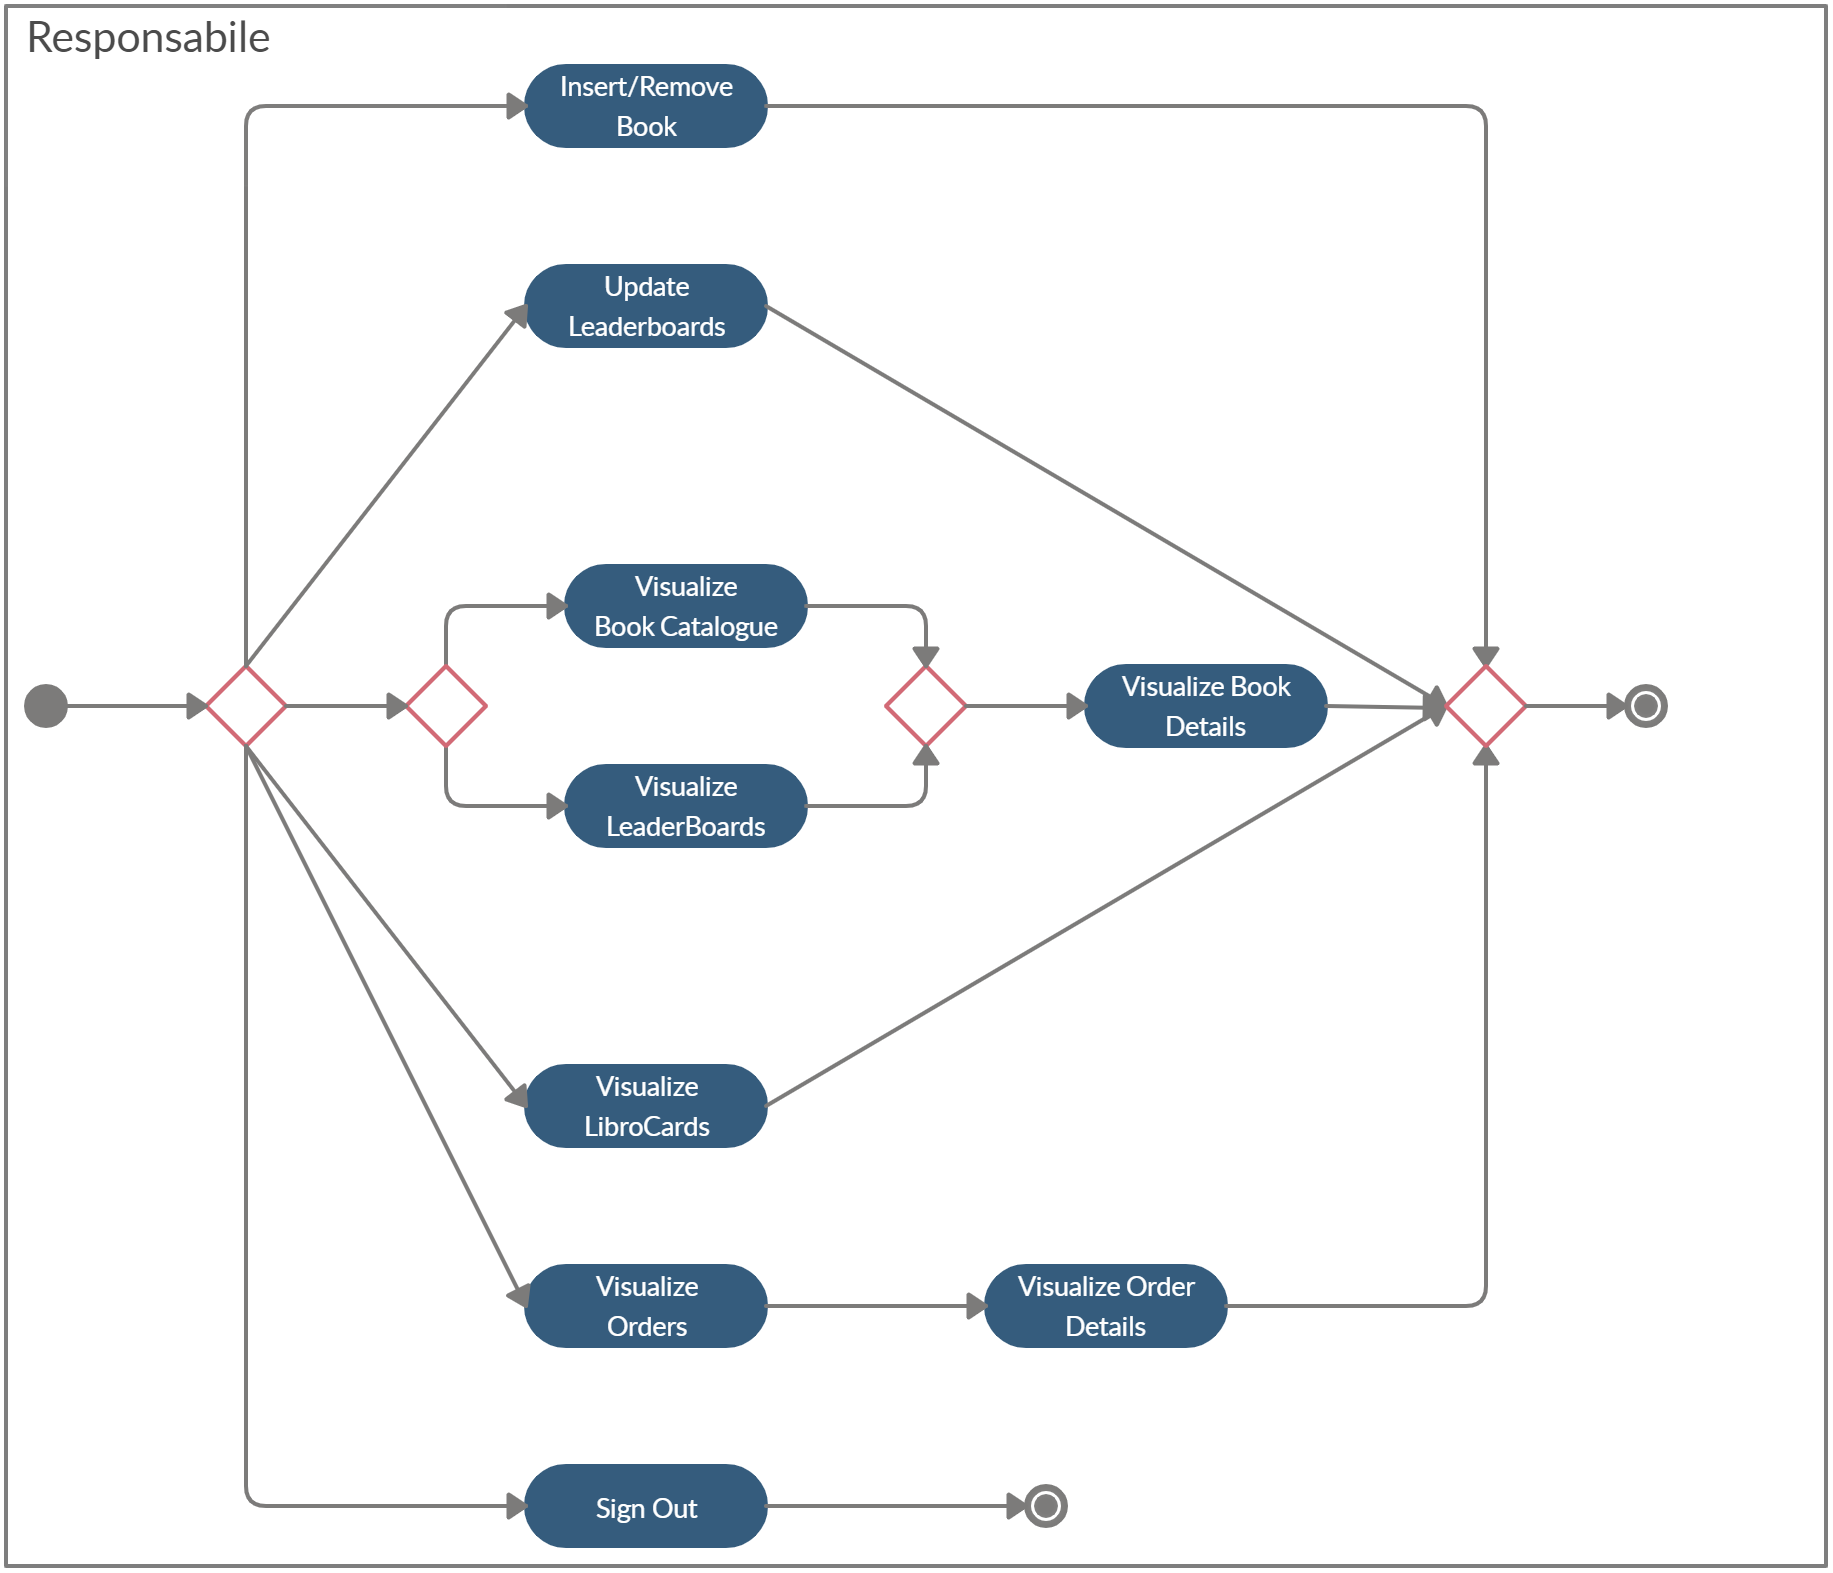
\includegraphics[scale=0.45, angle=90]{activityDiagramResponsabile}
		\caption{\textit{Activity diagram} delle diverse azioni che possono essere compiute dal responsabile}
\end{figure}
\cleardoublepage

\section{Sequence diagram}\label{sec:sequencediagram}
\begin{figure}[H]
		\centering
		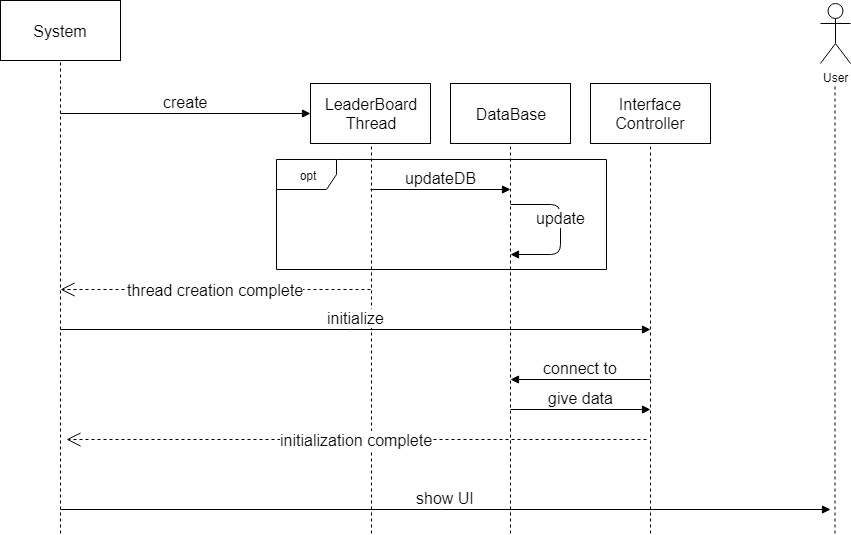
\includegraphics[scale=0.5]{sequenceDiagramBootPhase}
		\caption{\textit{Sequence diagram} delle operazioni eseguite durante il bootstrapping del sistema}
\end{figure}
\begin{figure}[H]
		\centering
		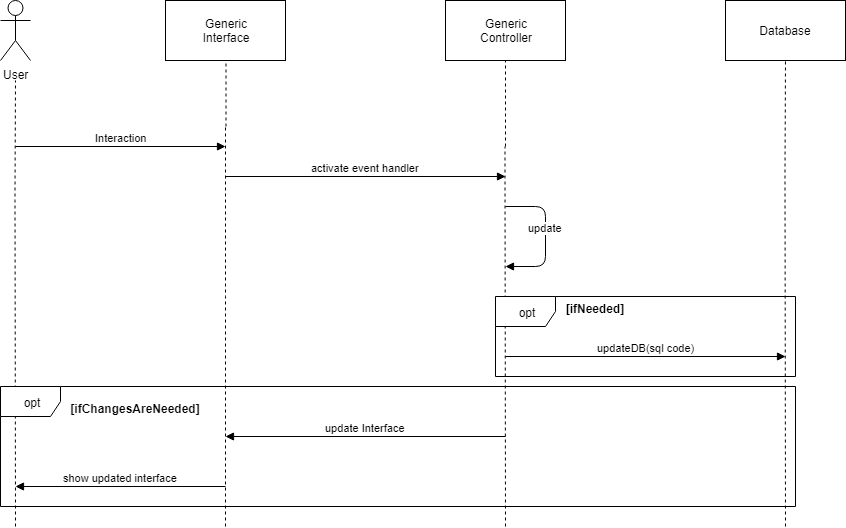
\includegraphics[scale=0.5]{sequenceDiagramGenericInteraction}
		\caption{\textit{Sequence diagram} che mostra le operazioni che avvengono a seguito di una generica interazione di un utente con il software}
\end{figure}
\begin{figure}[H]
		\centering
		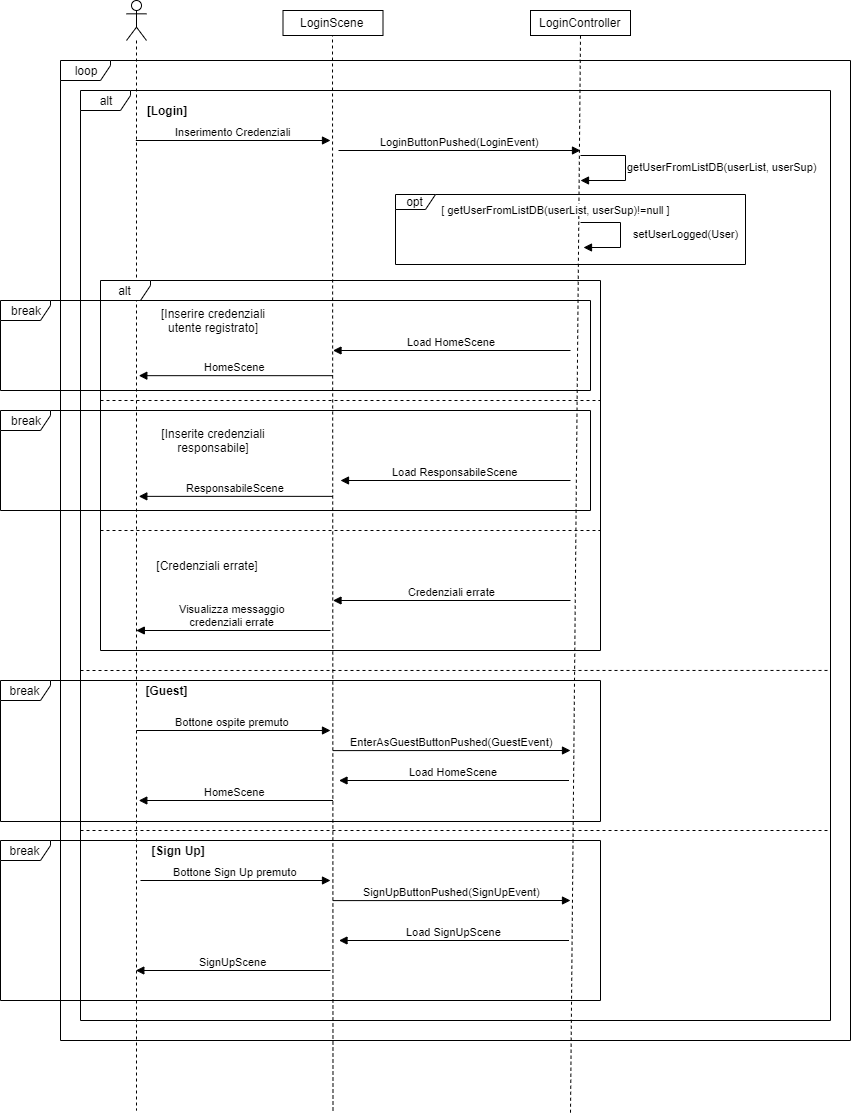
\includegraphics[scale=0.45]{sequenceDiagramLogin}
		\caption{\textit{Sequence diagram} delle diverse azioni che possono essere compiute nella schermata di Login}
\end{figure}

\section{Class diagram}\label{sec:calssdiagram}
\begin{figure}[H]
		\centering
		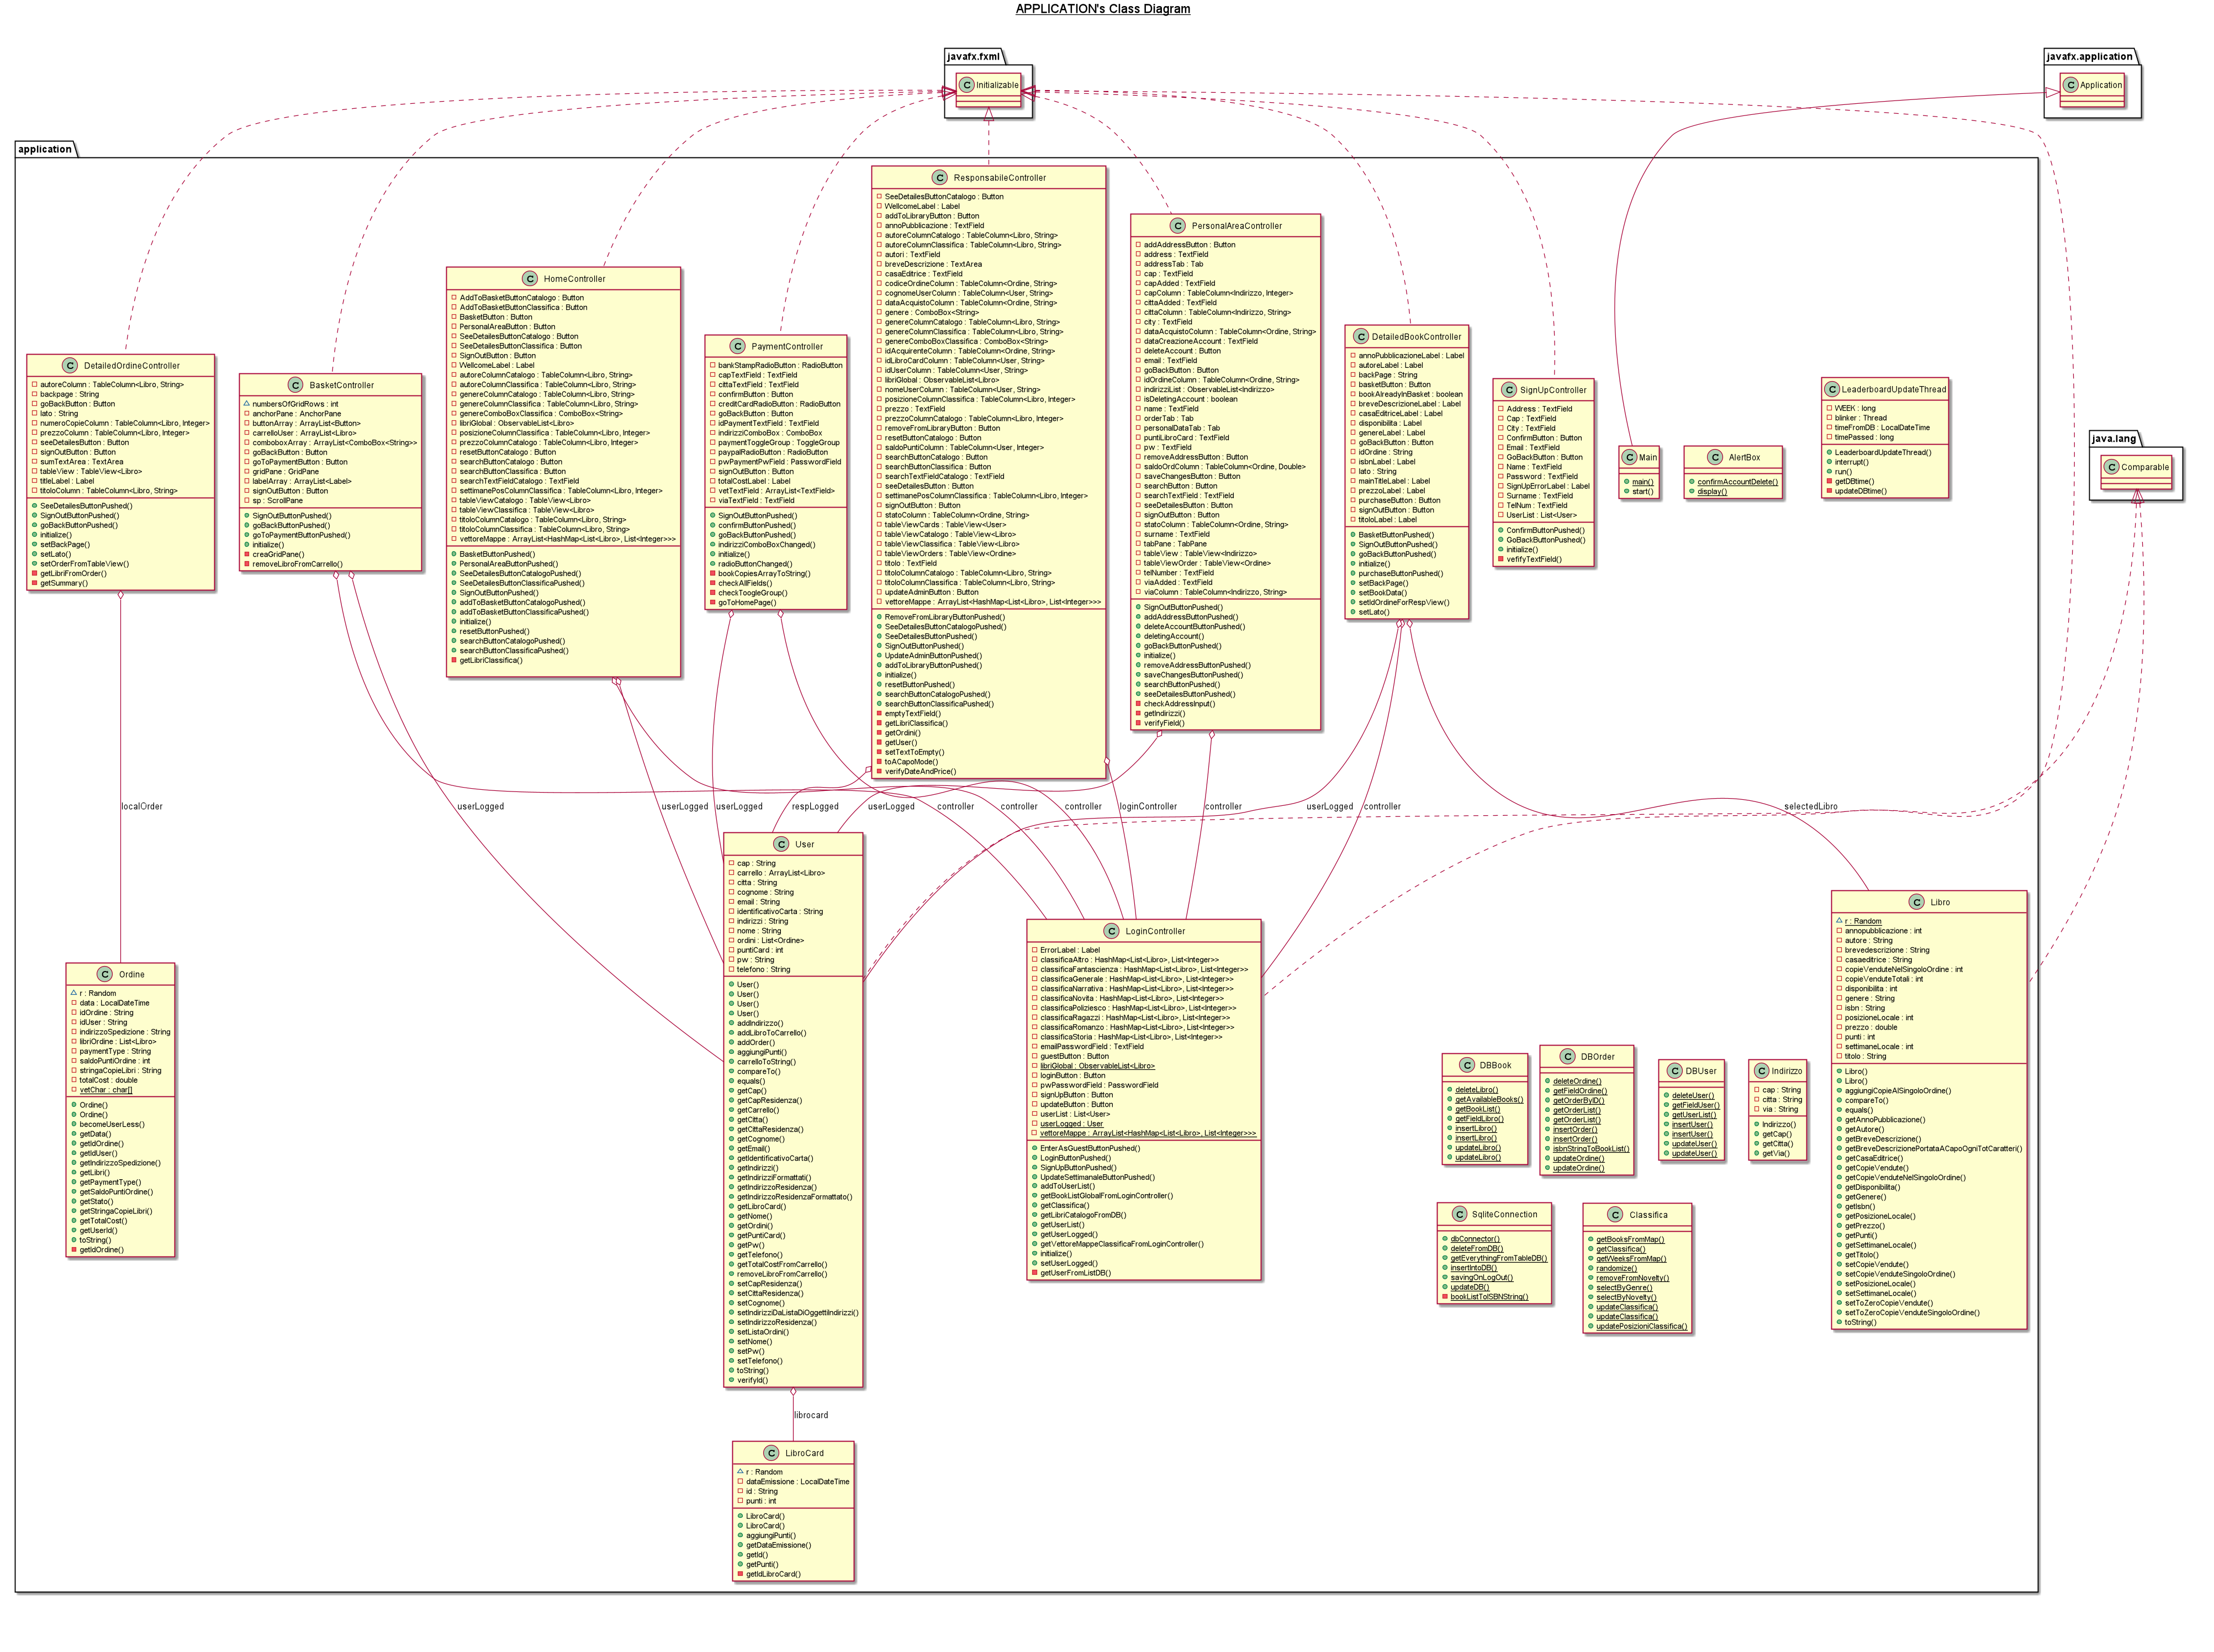
\includegraphics[scale=0.13, angle=90]{classDiagram}
		\caption{\textit{Class diagram} del sistema}
\end{figure}
\begin{figure}[H]
		\centering
		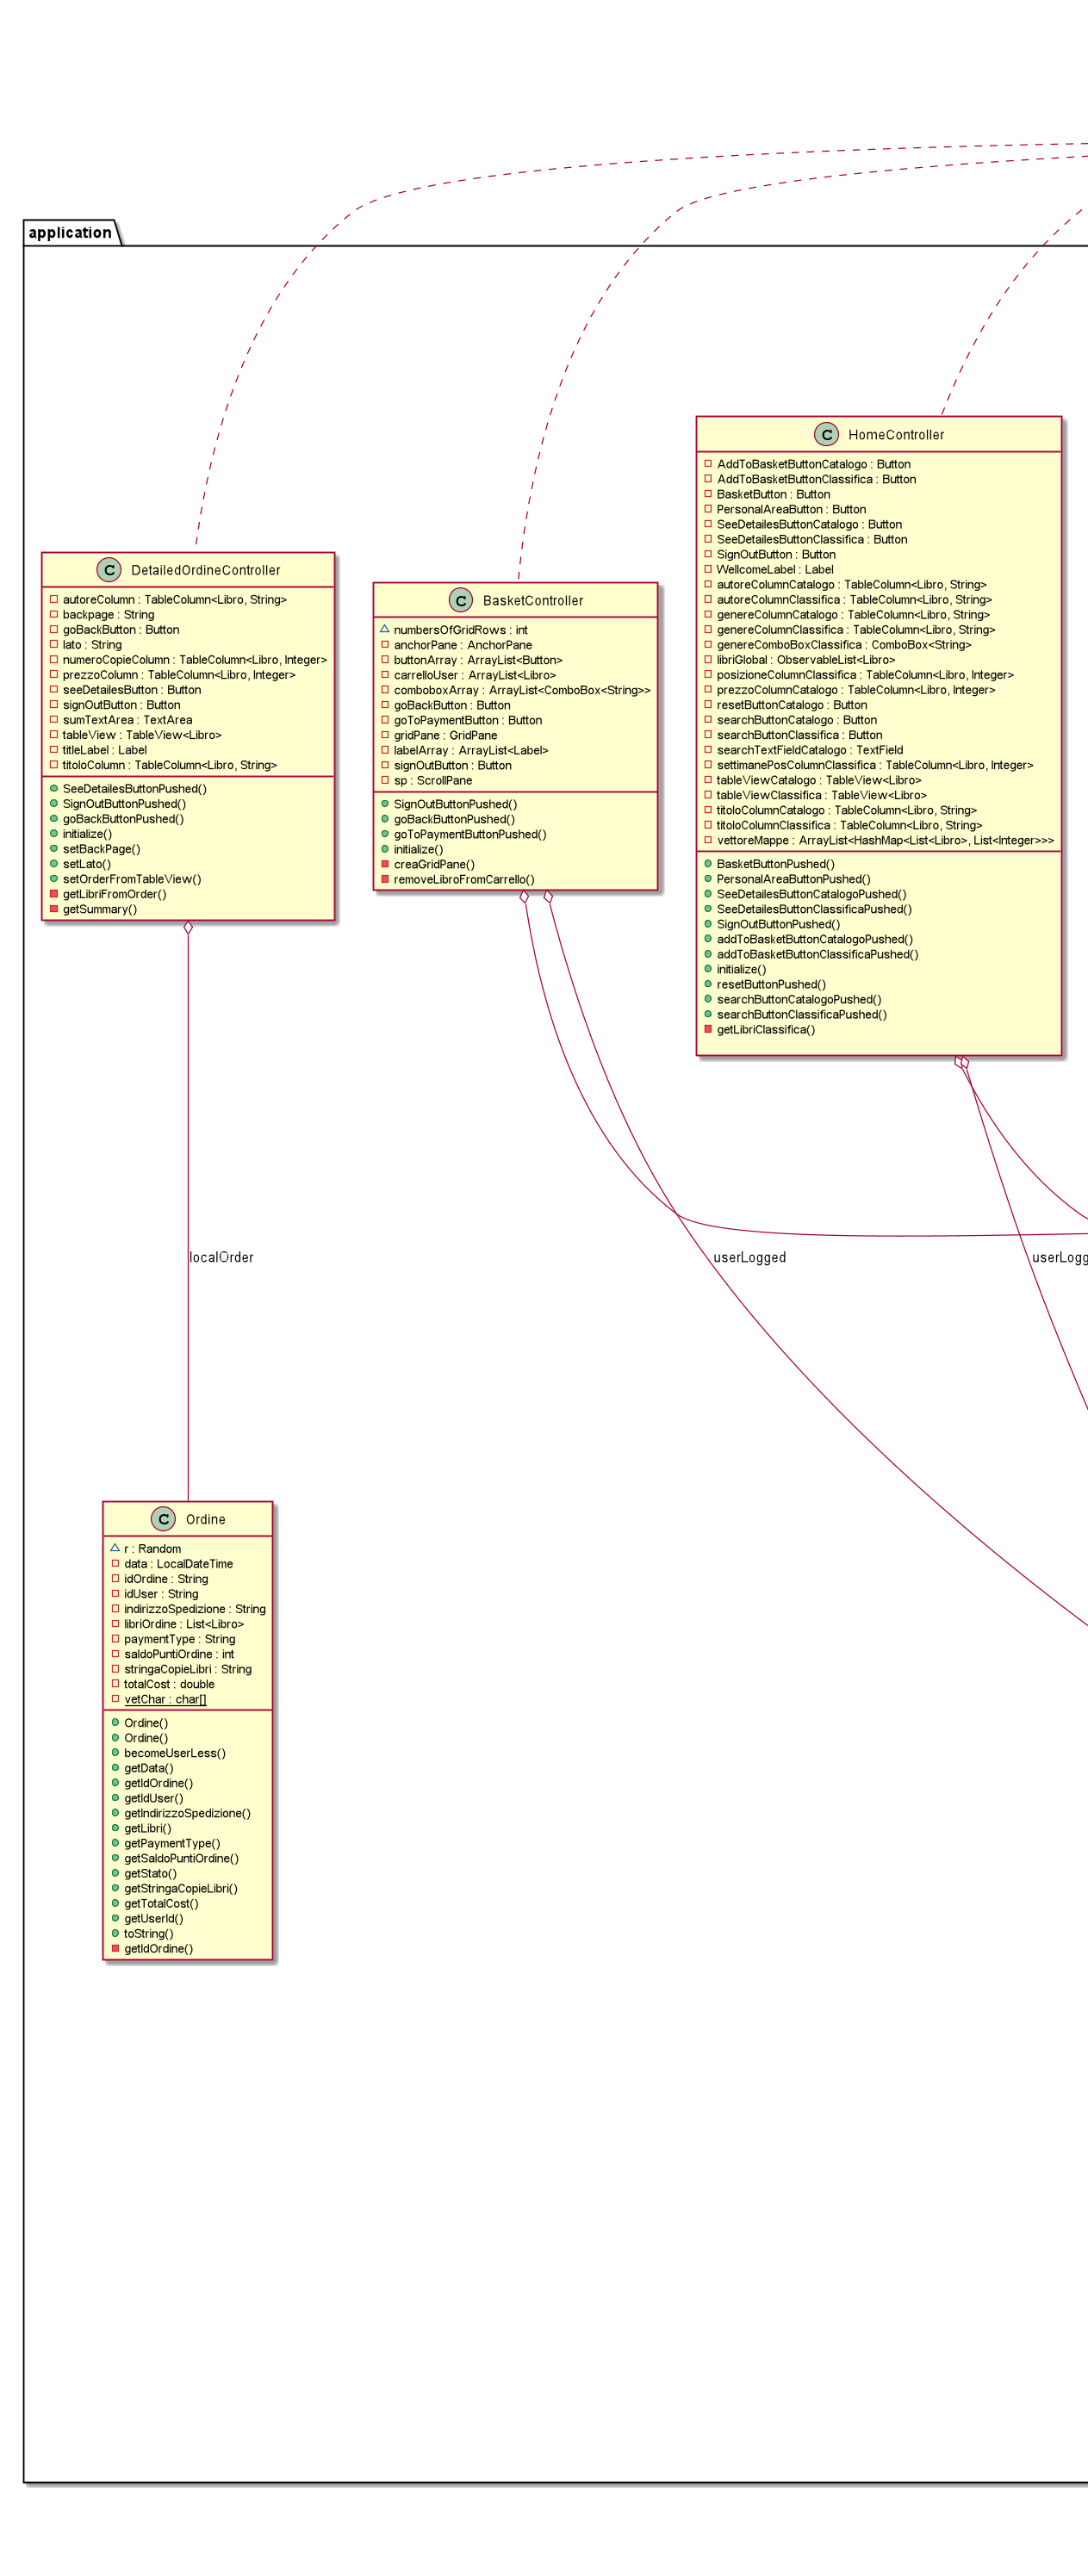
\includegraphics[scale=0.21]{classDiagramParte1}
\end{figure}
\begin{figure}[H]
		\centering
		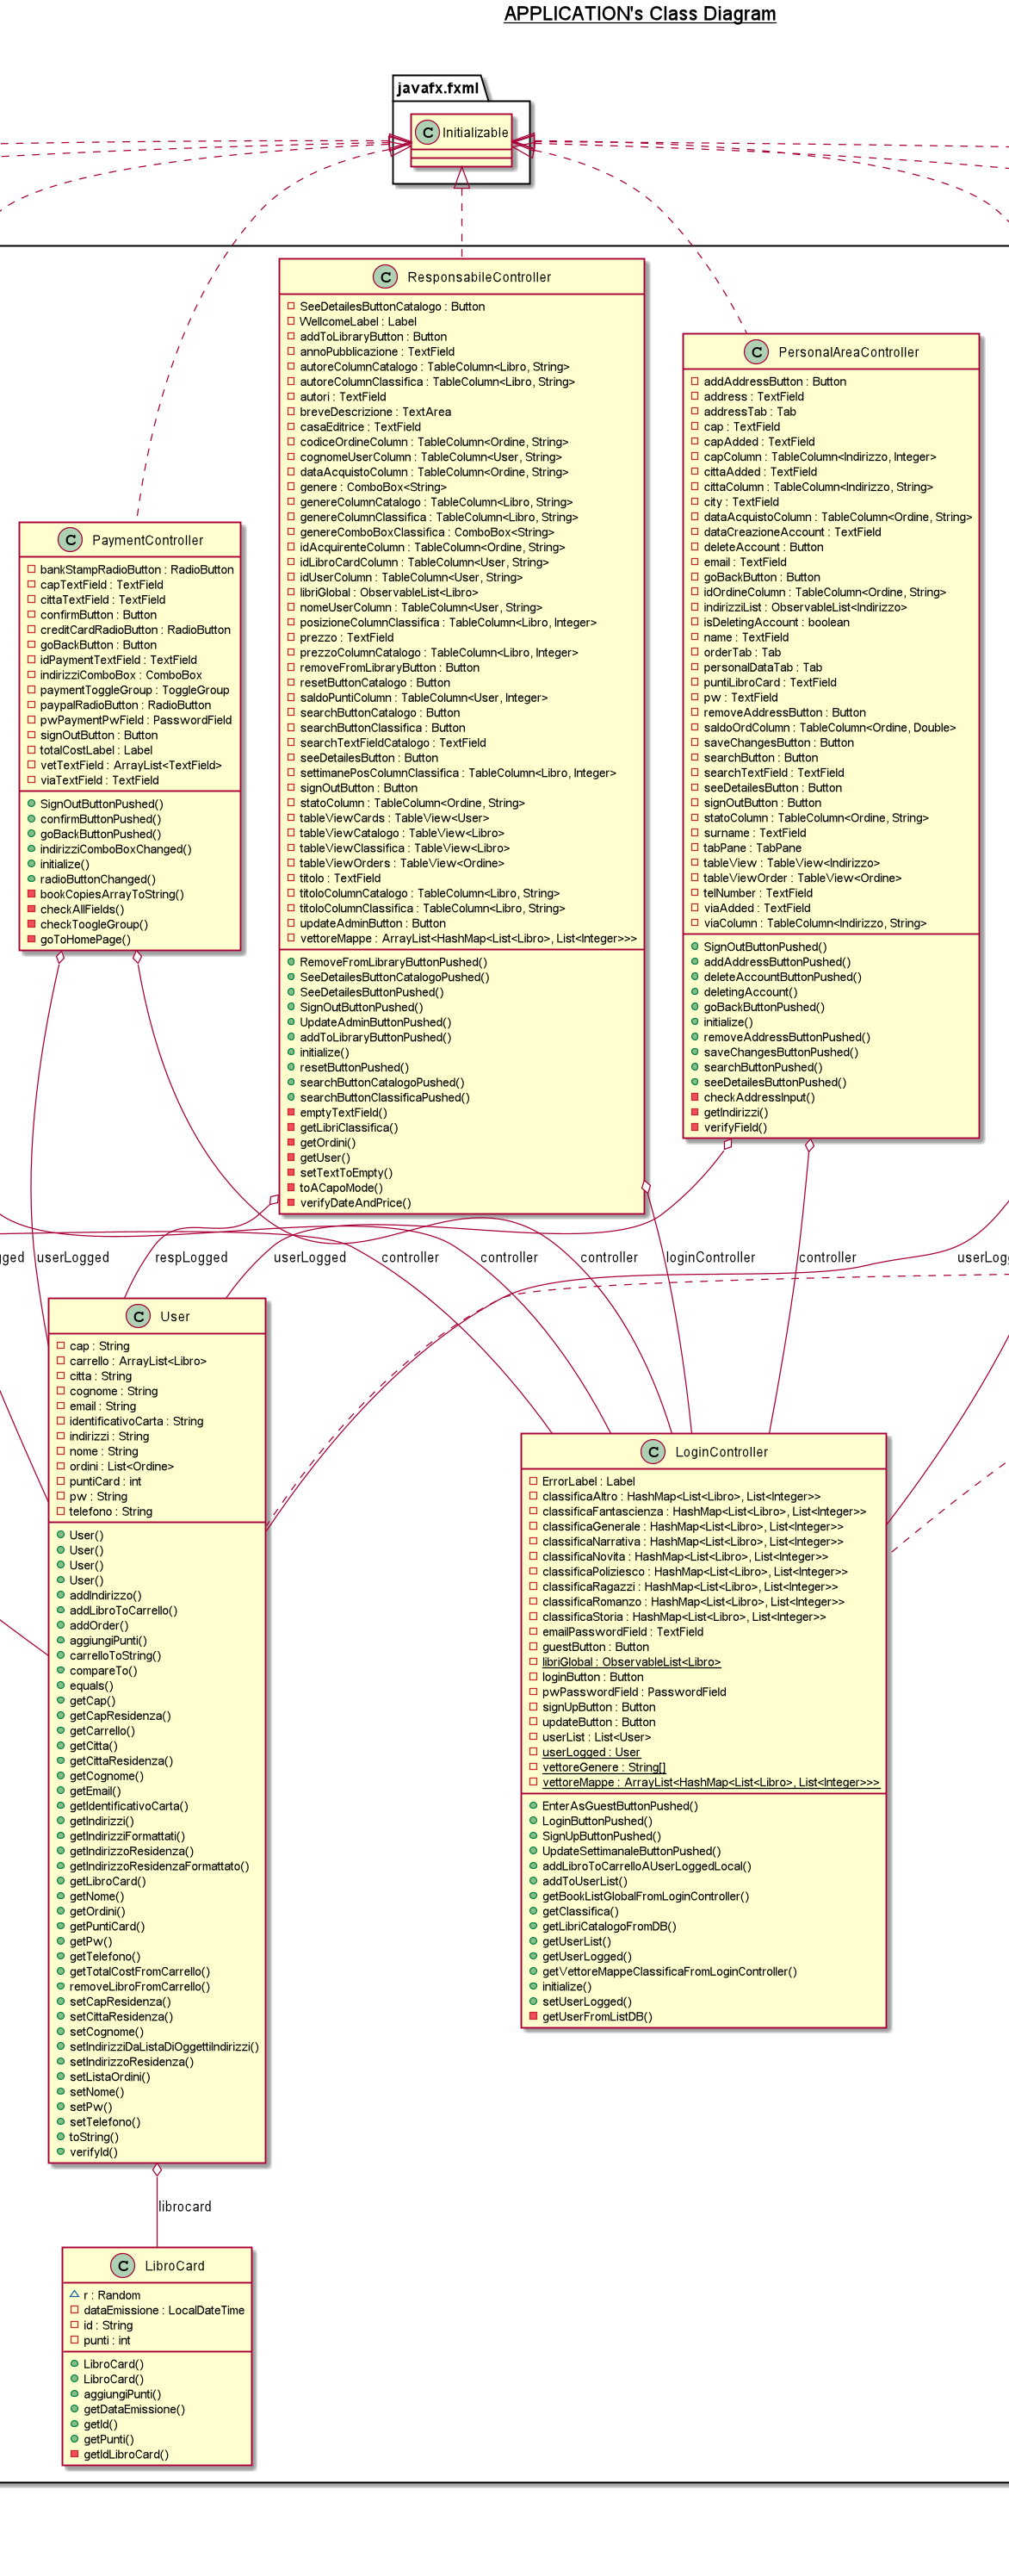
\includegraphics[scale=0.21]{classDiagramParte2}
\end{figure}
\begin{figure}[H]
		\centering
		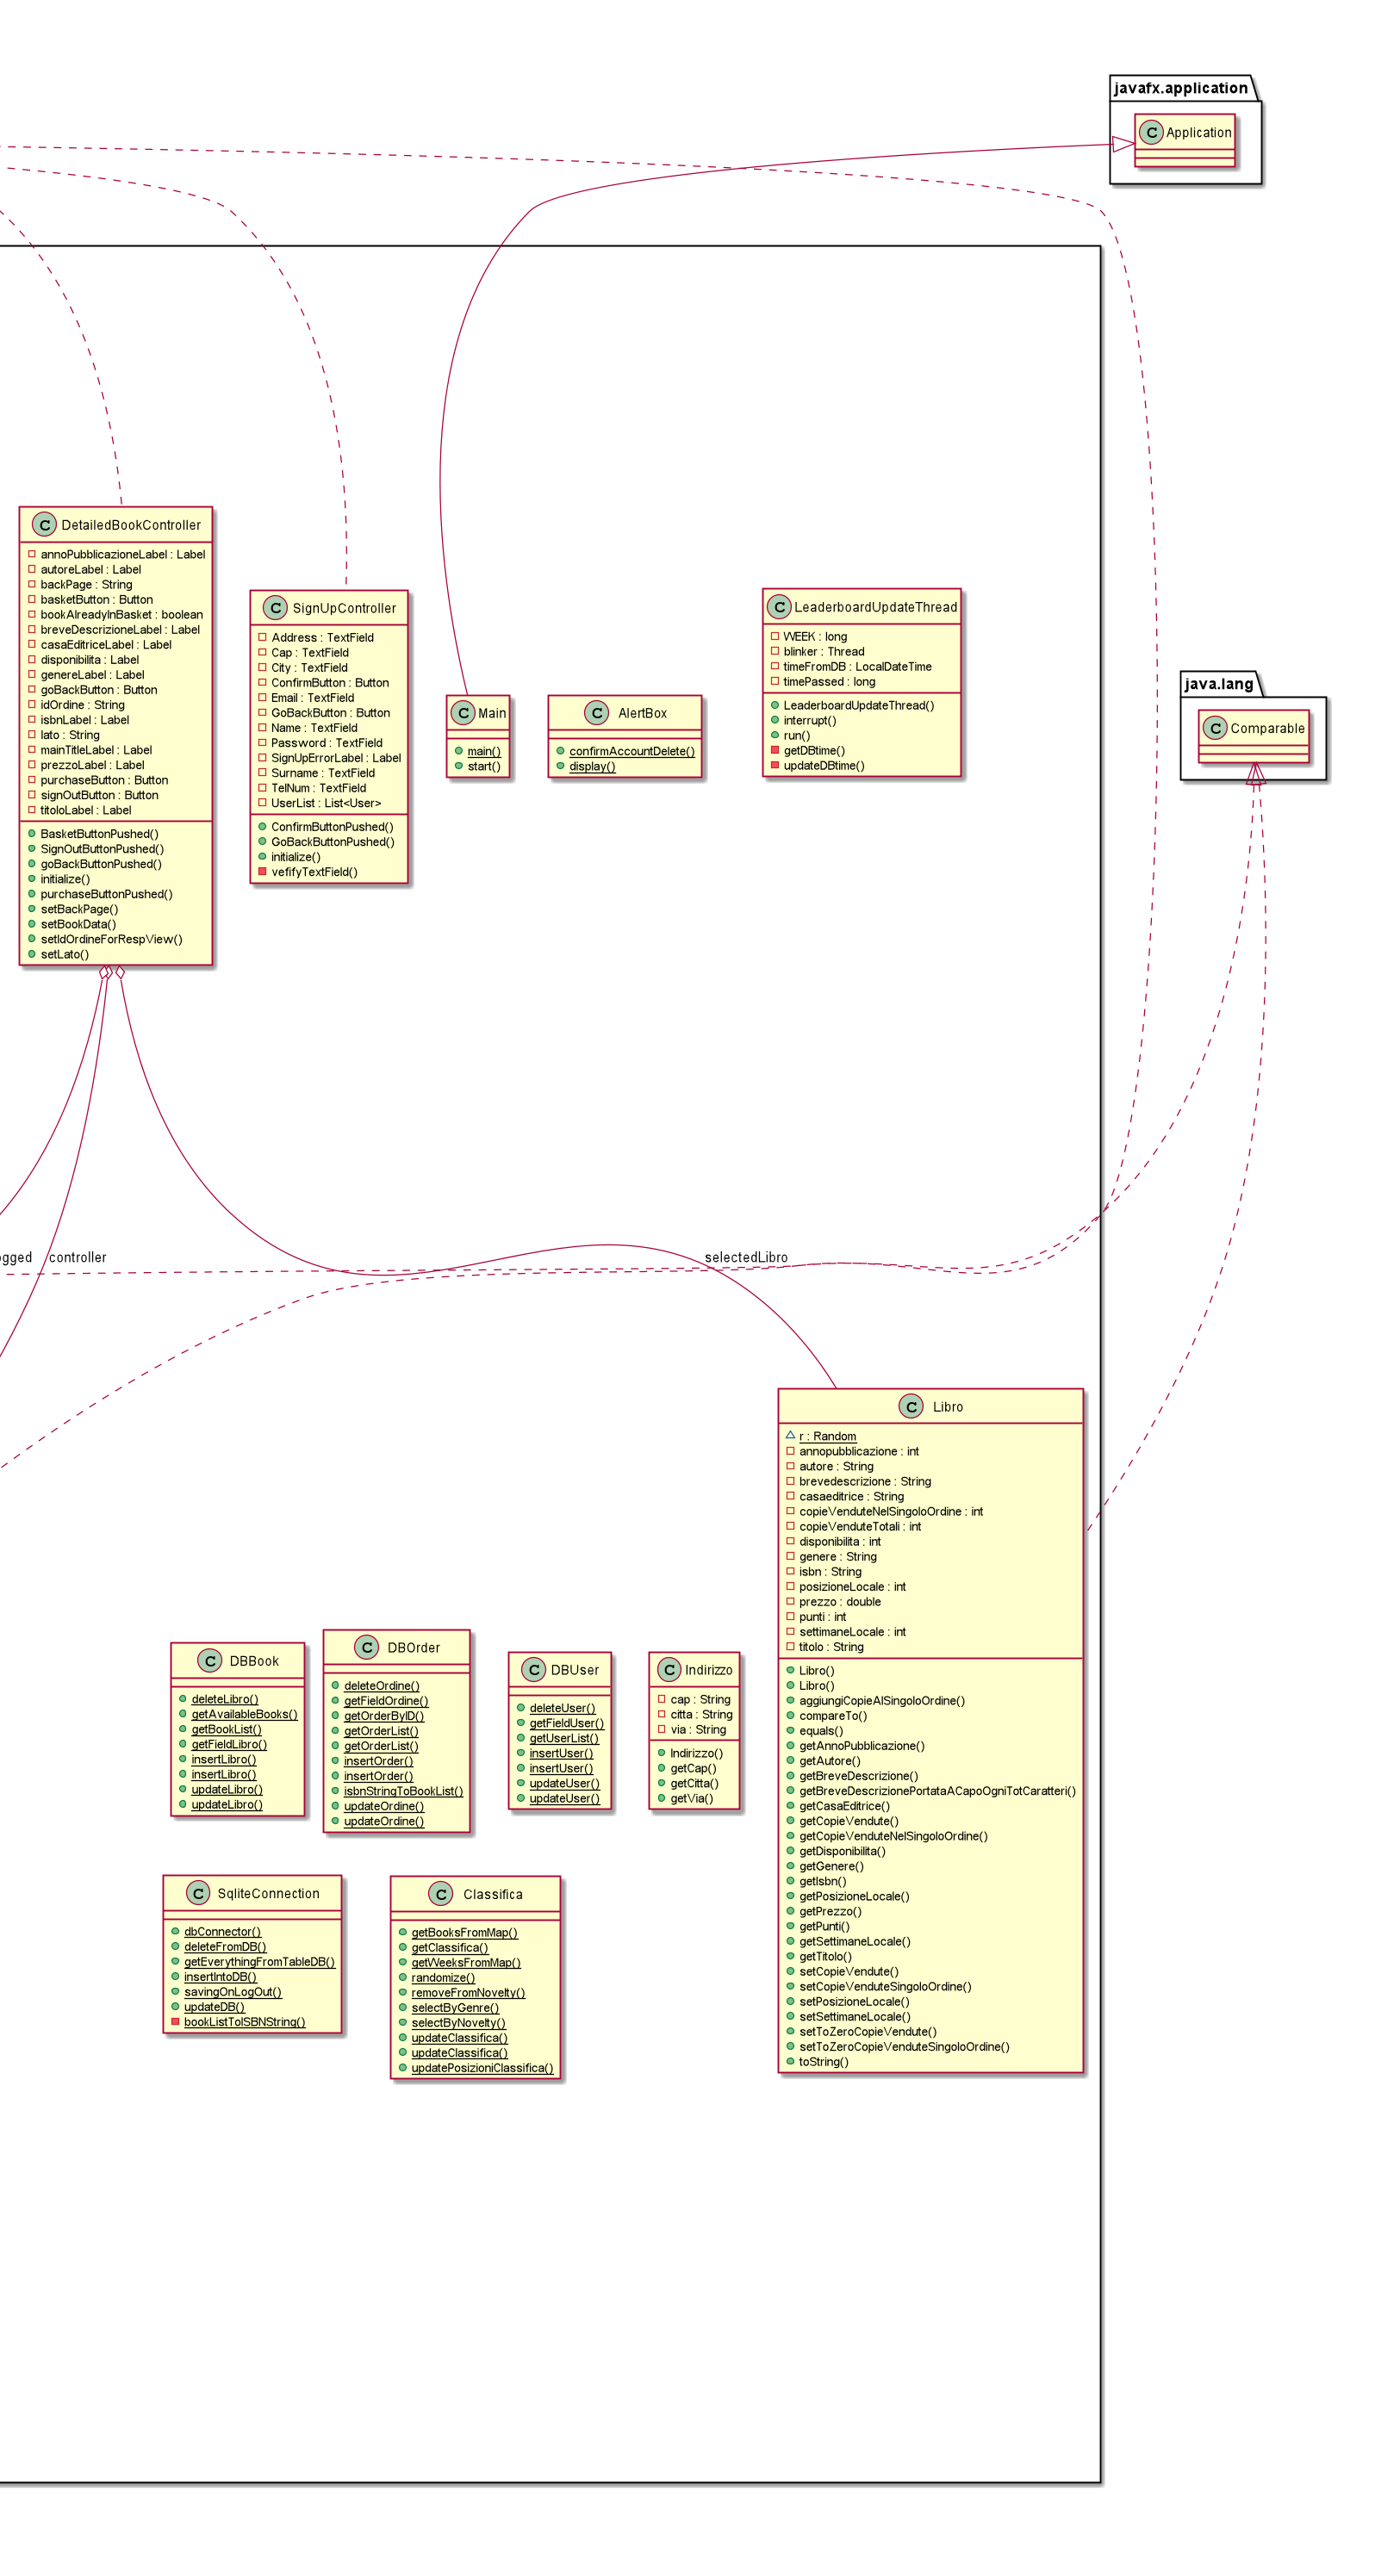
\includegraphics[scale=0.21]{classDiagramParte3}
\end{figure}
\section{Test e validazione}\label{sec:testevalidazione}
Durante lo sviluppo del progetto abbiamo innanzitutto testato il progetto (nelle singole parti o nella sua interezza) man mano che le componenti venivano sviluppate.\\ 
Una volta concluso il lavoro di codifica per prima cosa è stato di fondamentale importanza confrontare ciò che abbiamo prodotto con ciò che ci era stato richiesto. \\
Abbiamo quindi preso in esame la consegna e verificato che i diagrammi da noi prodotti rispettassero le specifiche del progetto.\\
In seguito abbiamo passato il codice visivamente, per verificare di aver applicato i pattern nel modo corretto.\\
Abbiamo poi iniziato a testare vari input e funzionamento dell'applicazione:
\begin{itemize}
\item Test sui singoli input, per verificare e quindi limitare l'inserimento dei dati nellle varie casistiche.
\item Test effettuati da noi stessi sull'intero progetto, per testare la possibilità di incongruenze o macroerrori.
\item Test effettuati da nostri compagni universitari, competenti in materia e vogliosi di trovare bachi.
\item Test effettuati da "persone normali" e dalle nostre madri, le quali dopo una prima fase di smarrimento nel non capire cosa avessero davanti, sono passate ad una seconda fase di smarrimento nel non capire la lingua con cui sono stati scritti i bottoni. E' stata una fase importante, vedere il progetto da un altro punto di vista (non tecnico) ci ha aiutato a dare un paio di ritocchi grafici per renderlo ancora più intuitivo.
\end{itemize}
\end{document}	